%
% Template for videoprojector foils according to the HZDR corporate design
% 
% (C) 2011 Alexander Grahn, HZDR, Institut fuer Sicherheitsforschung
%
% Version 20131126
%
\documentclass[
%  aspectratio=43, %default screen size (4:3); other values: 1610, 169, 149, 54, 32
%  smaller, %uncomment this to fit more text onto the slides (similar to the CD suggestions)
  intlimits %put limits of integrals above and below the integral symbol
]{beamer}

%\usepackage[ngerman]{babel}
\usepackage[UKenglish]{babel}

%my favourite packages
\usepackage[latin1]{inputenc} %type in accented characters easily, i. e. � instead of \"a 
%\usepackage{siunitx} %easy input & nice formatting of phys. quantities (number + SI unit)
%\usepackage{latexsym}
%\usepackage{amssymb}
\usepackage{media9}
%\usepackage{animate}
\usepackage{ragged2e}\RaggedRight
\usepackage{fancyvrb}
\usepackage{ifthen}

%%%%%%%%%%%%%%%%%%%%%%%%%%%%% some optional settings %%%%%%%%%%%%%%%%%%%%%%%%%%%%%%%%%%%%
%uncomment this if you want the title page text aligned flushleft; CD rules seem to
%demand this, although it looks awful
%\def\titleflushleft{}

%uncomment this if you want frame titles centred
%\def\frametitlecentered{}

%uncomment this if you don't like the wallclock
%\def\noclock{}

%uncomment this if you don't like the navigation buttons
%\def\nonavigation{}

%uncomment this if you want Arial as the main text font (very ugly),
%no matching math font, using CM-Bright for math text
%\def\arial{}

%uncomment this if you want Helvetica as the main text font (very ugly),
%Helvetica is very similar to Arial; again, no matching math font, using CM-Bright for
%math text
%\def\helvetica{}

%hzdr colours used for various text highlights; see manual `beameruserguide.pdf',
%chapter 12 for further possibilities
                                               %colour will be used in:
\setbeamercolor{alerted text}{fg=hzdr-orange}  %\alert{text to be highlighted},
                                               %\begin{alertenv} ... \end{alertenv}
                                               %\begin{alertblock}{block title (highlighted)}
                                               %  ...
                                               %\end{alertblock}

\setbeamercolor{example text}{fg=hzdr-darkblue}%\begin{exampleblock}{block title (highlighted)}
                                               %  ...
                                               %\end{exampleblock}
%%%%%%%%%%%%%%%%%%%%%%%%%%%%%%%%%%%%%%%%%%%%%%%%%%%%%%%%%%%%%%%%%%%%%%%%%%%%%%%%%%%%%%%%%

%hzdr theme
\makeatletter
\def\input@path{{beamerthemehzdr/}}
\makeatother
\usetheme{hzdr}

%%%%%%%%%%%% title, author, date, institute, additional logos %%%%%%%%%%%%%%%%%%%%%%%%%%%
\title{HASEonGPU}
\subtitle{An Open-Source ASE code for calculating the gain in high power laser media on GPU clusters}% may be left empty, of course

%[short version of authors to be used in footlines]{long version in the title page}
\author[C. Eckert, E. Zenker et al.]{
\texorpdfstring{\underline{Carlchristian Eckert}\inst{1}}{},
\texorpdfstring{\underline{Erik Zenker}\inst{1}}{}
}


%\date{\today}
\date{15th July 2014}

\institute[
 %short version of main authors' institute, used in the footline
 \iflanguage{ngerman}{%
   Institut f�r Strahlenphysik%
 }{%
   Institute of Radiation Physics%
 }%
]{%
 %used in the title page
 \iflanguage{ngerman}{%
   \inst{1}Helmholtz-Zentrum Dresden-Rossendorf, Institut f�r Strahlenphysik\\
 }{%
   \inst{1}Helmholtz-Zentrum Dresden-Rossendorf, Institute of Radiation Physics\\
 }%
}

%every invocation of the macro \partnerlogo{...} adds YET ANOTHER partner logo to the
%right of the already inserted partner logos;
%the starred version `\partnerlogo*{}' inserts s-t-r-e-t-c-h-a-b-l-e space between the current
%logo and the next one on its right side: this allows for logos/groups of logos to be
%aligned flush-left on the page
%\partnerlogo*{\colorbox{gray}{\tiny Logo 1}}% some logo
\partnerlogo{
  \ifthenelse{\theframenumber=0}{%  %title slide
    
\includegraphics[height=0.14\paperheight]{graphics/haseOnGPU.png}
  }{
    
\includegraphics[height=0.06\paperheight]{graphics/haseOnGPU.png}
  }
}
\partnerlogo{
  \ifthenelse{\theframenumber=0}{%  %title slide
    
\includegraphics[height=0.1\paperheight]{graphics/ccoe_small.png}
  }{
    
\includegraphics[height=0.05\paperheight]{graphics/ccoe_small.png}
  }
}
\partnerlogo{% DD-concept logo; note that different versions are used on title and normal slides
  \ifthenelse{\theframenumber=0}{%  %title slide
    
\includegraphics[height=0.08\paperheight]{DDC-weisse-schrift}%
  }{%                               %normal slides
    
\includegraphics[height=0.05\paperheight]{DDC-orig}%
  }%
}
%%%%%%%%%%%%%%%%%%%%%%%%%%%%%%%%%%%%%%%%%%%%%%%%%%%%%%%%%%%%%%%%%%%%%%%%%%%%%%%%%%%%%%%%%%

\hypersetup{%
  breaklinks,colorlinks,
  %pdfpagemode=FullScreen,
  pdfhighlight=/P,
  linkcolor=hzdr-darkblue,
  linkcolor=hzdr-darkblue,
  anchorcolor=hzdr-darkblue,
  citecolor=hzdr-darkblue,
  filecolor=hzdr-darkblue,
  menucolor=hzdr-darkblue,
  runcolor=hzdr-darkblue,
  urlcolor=hzdr-darkblue
}

%\newcommand{mycom}[2]{}

\begin{document}

\newcommand{\myuncover}[2]{\uncover<{#1}-{#2}>}
\newcommand{\myonly}[1]{\only<{#1}>}
%\renewcommand{\myuncover}[2]{}
%\renewcommand{\myonly}[1]{}

\frame{\titlepage}

\autobookmark
\begin{frame}[t]{Amplified Spontaneous Emission is a fundamental process in laser physics}
  \myonly{1}{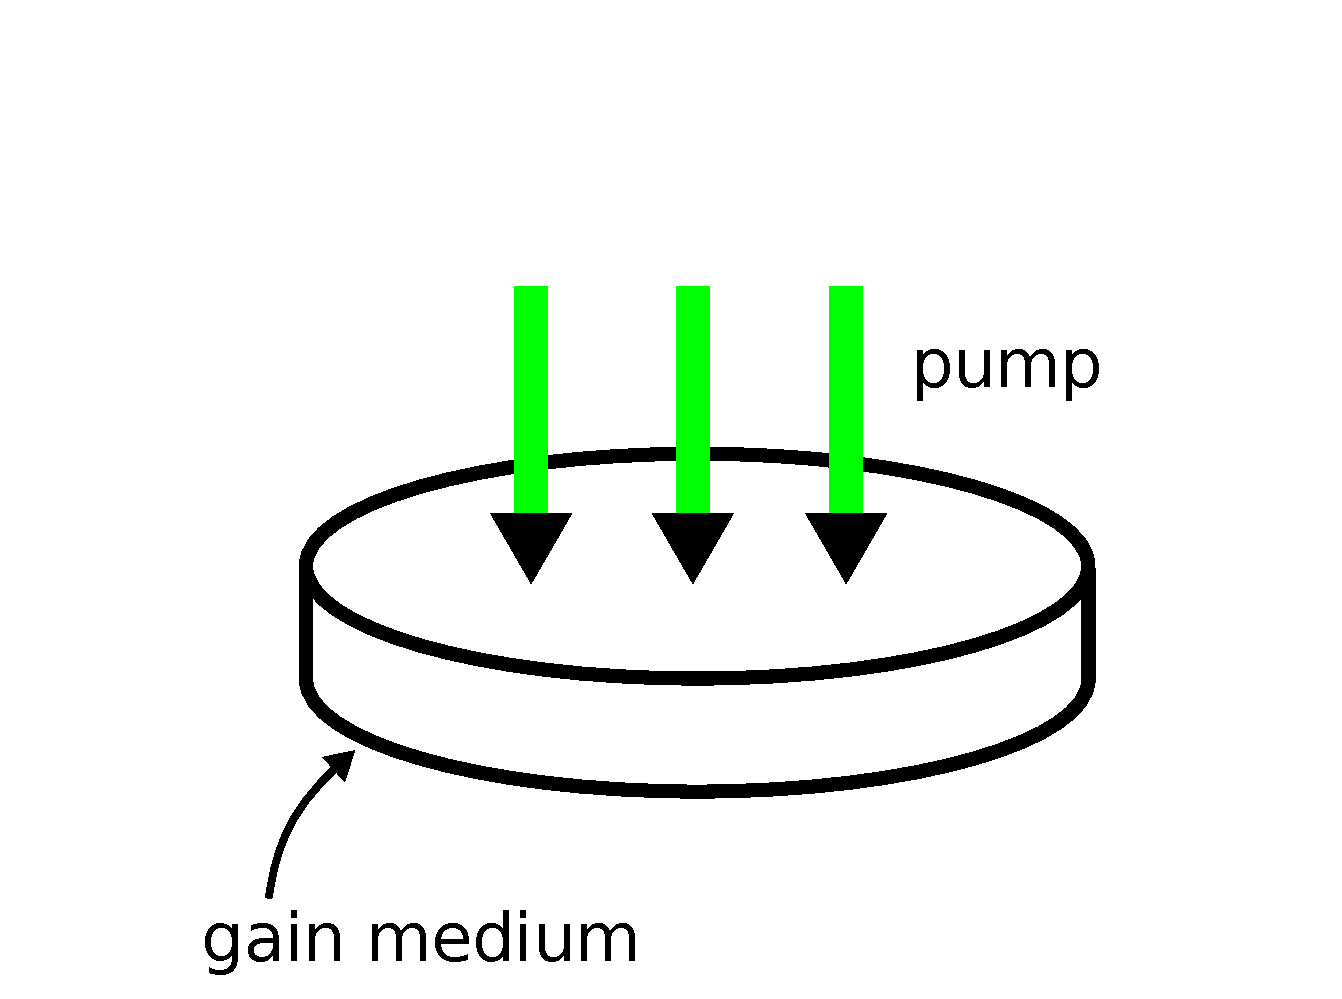
\includegraphics[width=0.8\paperwidth]{graphics/gain_medium_pumped_0.pdf}}
  \myonly{2}{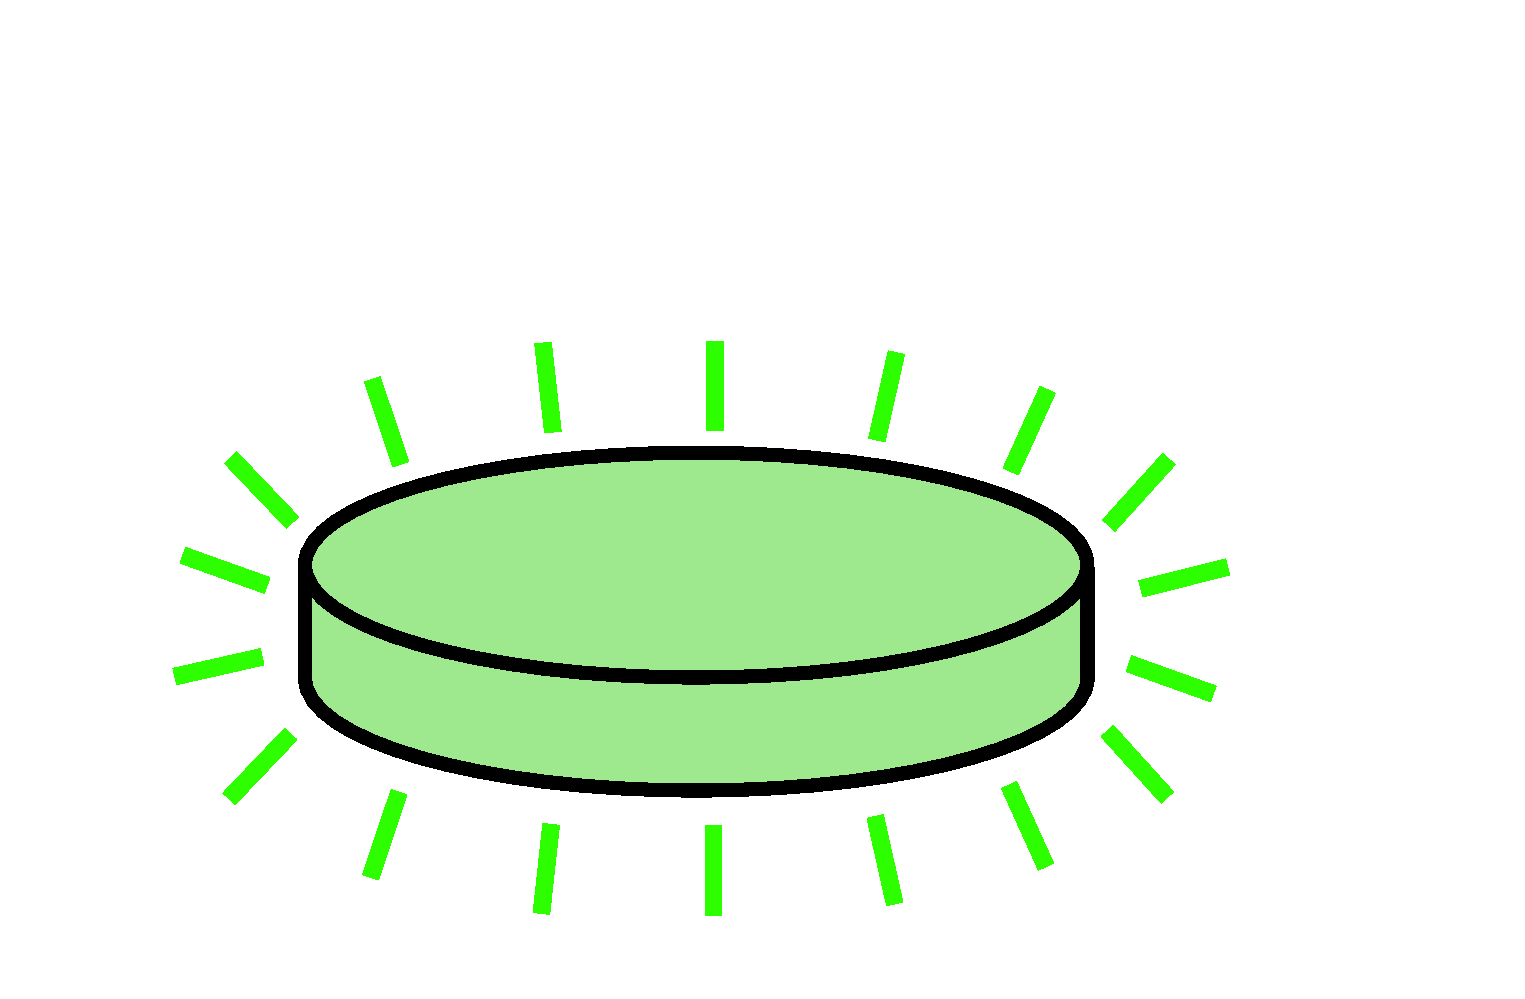
\includegraphics[width=0.8\paperwidth]{graphics/gain_medium_pumped_1.pdf}}
  \myonly{3}{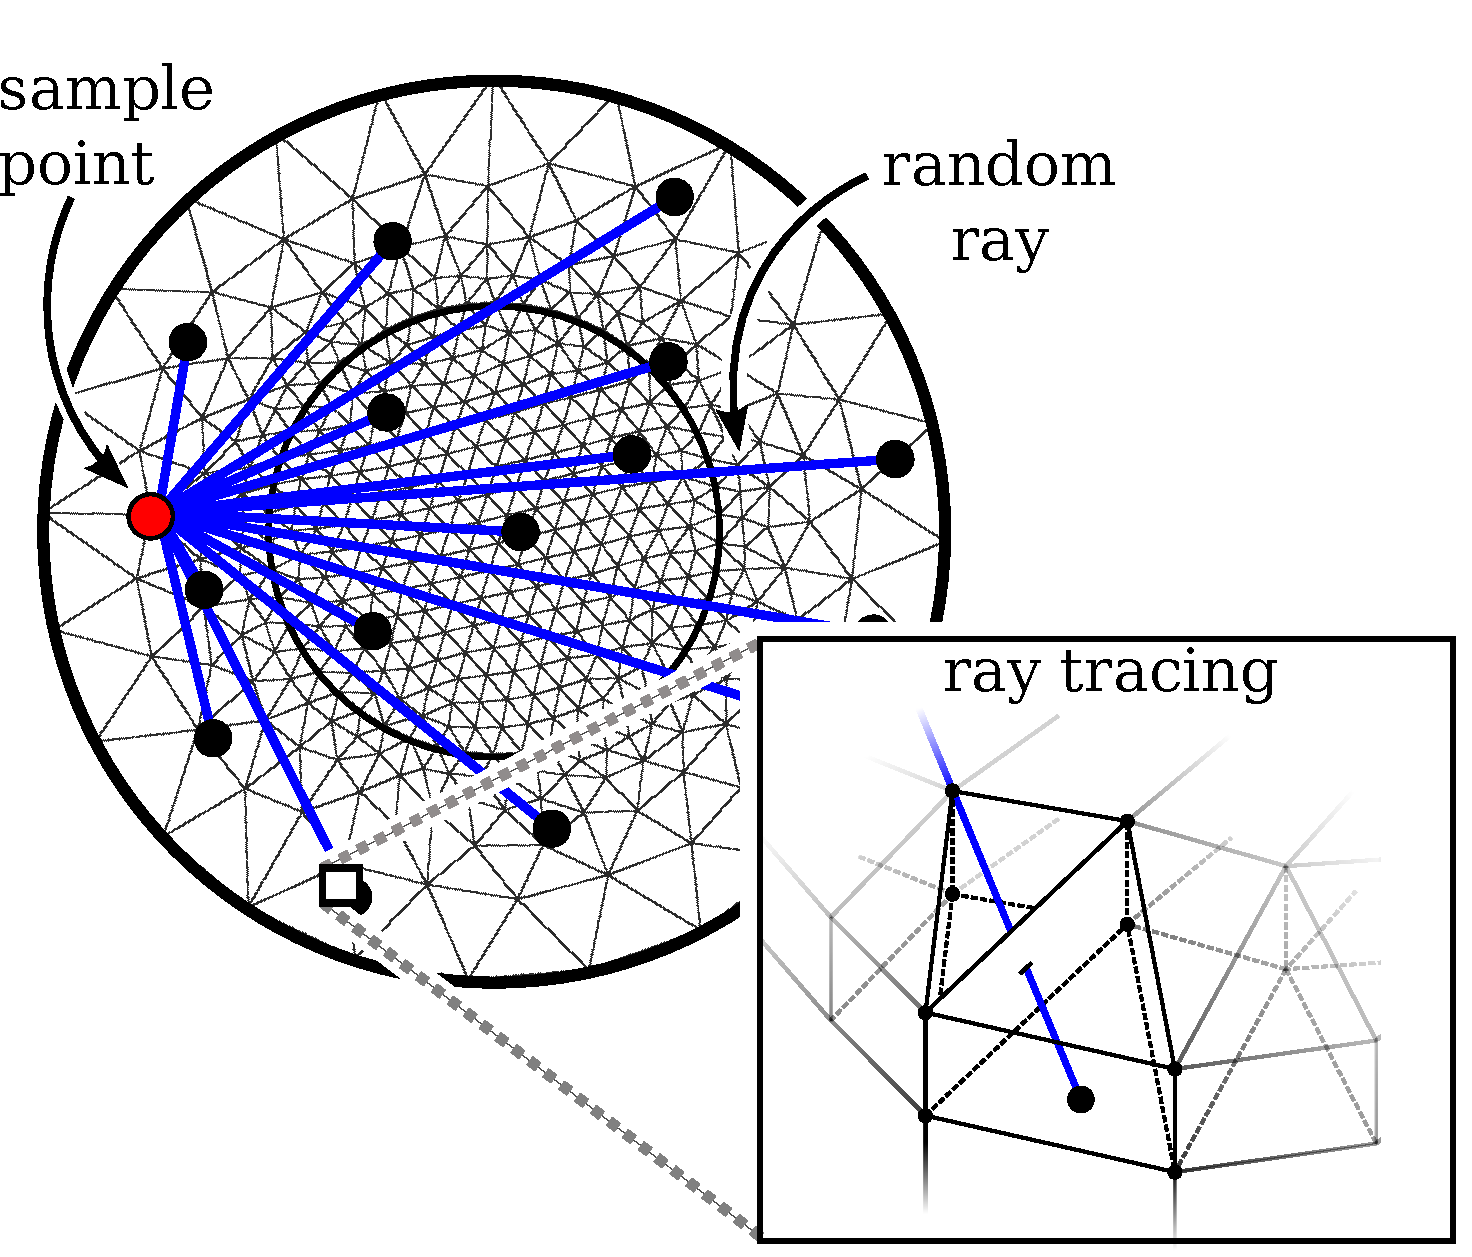
\includegraphics[width=0.8\paperwidth]{graphics/gain_medium_pumped_2.pdf}}
  \myonly{4}{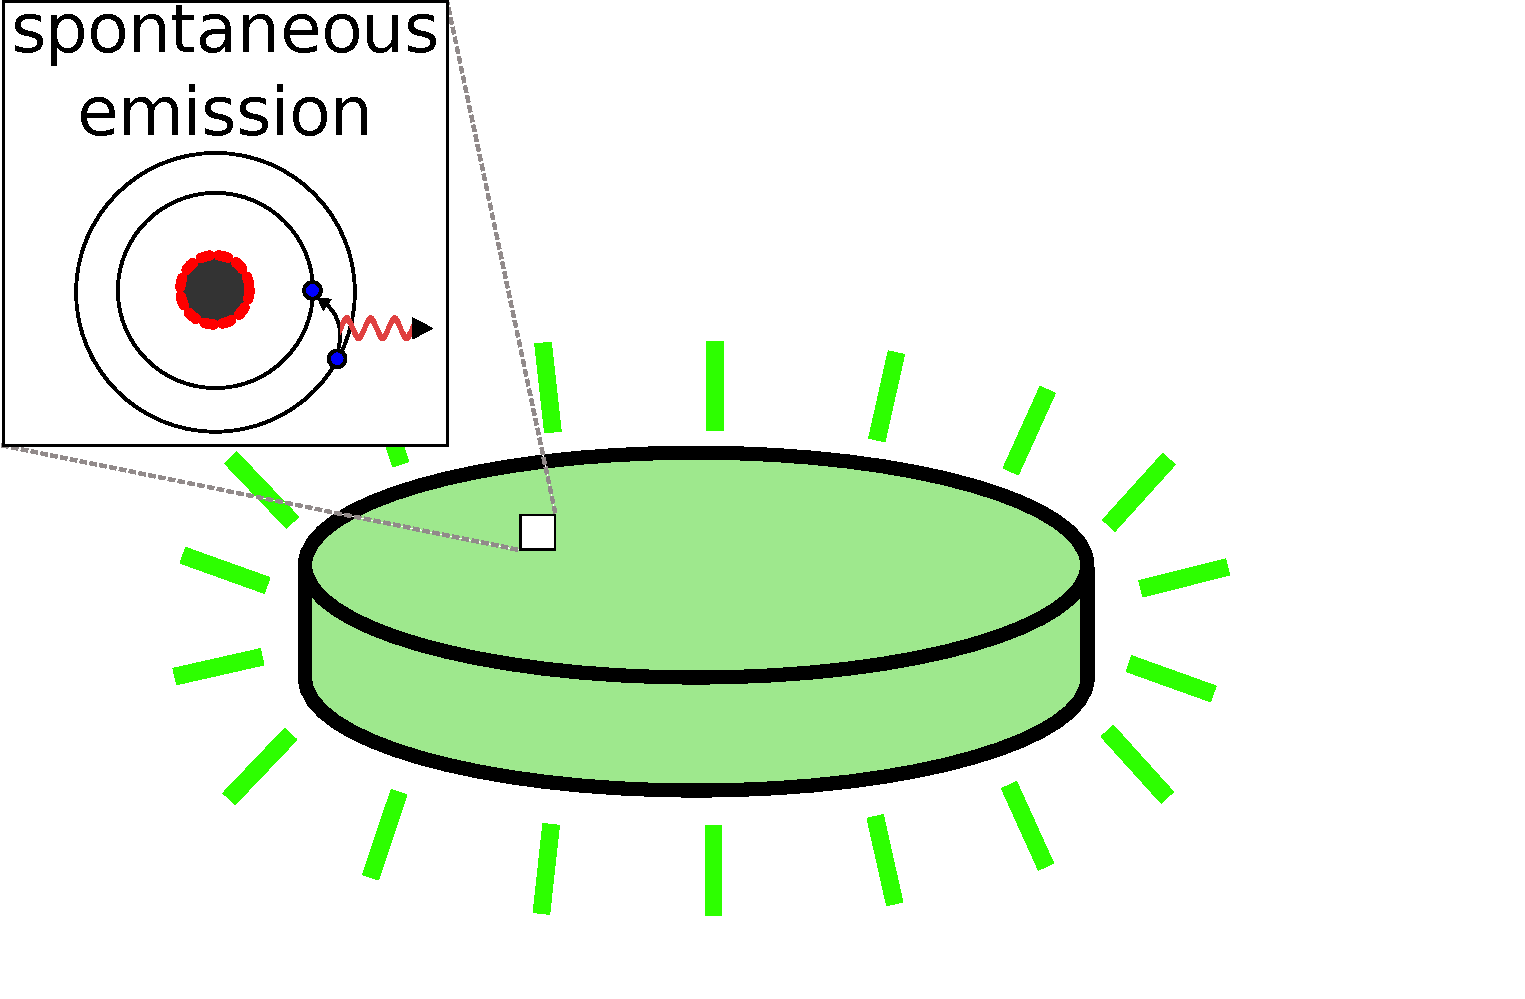
\includegraphics[width=0.8\paperwidth]{graphics/gain_medium_pumped_3.pdf}}
  \myonly{5}{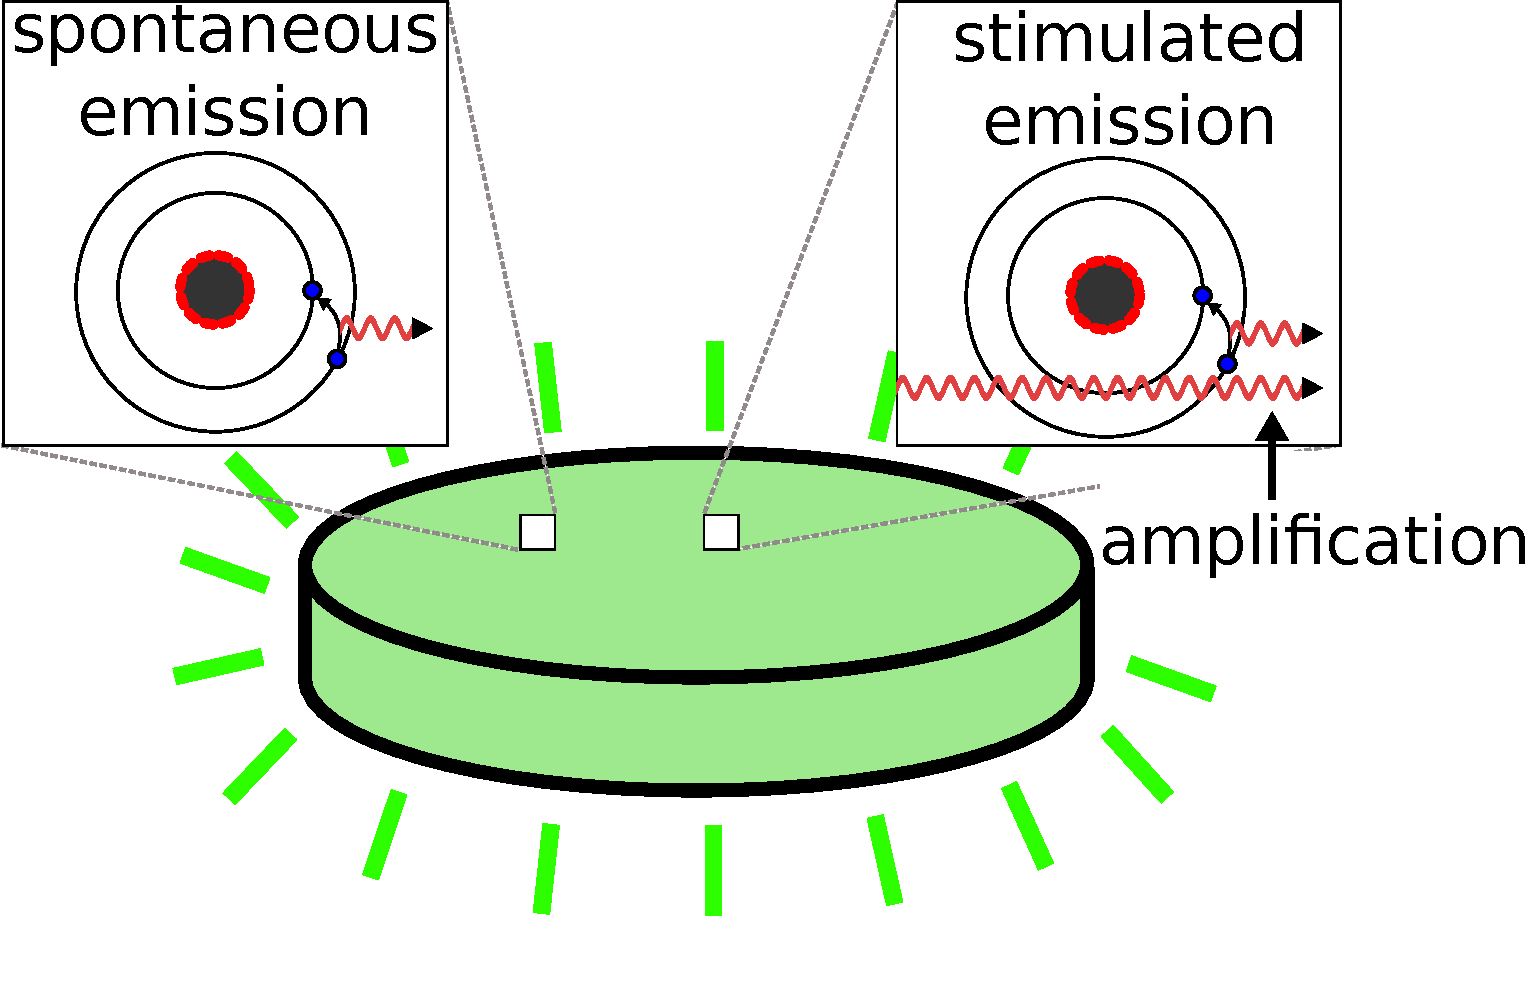
\includegraphics[width=0.8\paperwidth]{graphics/gain_medium_pumped_4.pdf}}
%
%  \begin{columns}[T]
%
%    \begin{column}{.5\textwidth}
%      \textbf{graphic: ASE crystal, with a photon travelling through it?}\\[2ex]
%      \textbf{alternative: laser setup, pumping a gain medium?}
%    \end{column}
%
%    \begin{column}{.5\textwidth}
%      \begin{itemize}
%      \myuncover{1}{3}{
%        \item In laser physics, gain media are pumped by lasers\\[1ex]
%      }
%      \myuncover{2}{3}{
%        \item Over time, electrons fall back into lower energy levels, causing
%          the spontaneous emission of a photon\\[1ex]
%      }
%      \myuncover{3}{3}{
%        \item Photon travels through the medium, where it is amplified by more
%          photons that are released
%      }
%  \end{itemize}
%    \end{column}
%
%  \end{columns}
\end{frame}

\autobookmark

\begin{frame}{Simulation of ASE is required for better laser design}
  \begin{columns}[T]

    \begin{column}{.5\textwidth}
    \myuncover{1}{3}{\textbf{graphic: plot of gain-experiment}\\[2ex]}
    \myuncover{2}{3}{\textbf{graphic: time developement of gain medium}}
    \end{column}

    \begin{column}{.5\textwidth}
      \begin{itemize}
          \myuncover{1}{3}{
          \item Amplified Spontaneous Emission limits the amount of energy
            stored in the gain medium\\[1ex]
          }
          \myuncover{3}{3}{
          \item Precise simulation of ASE is needed to design energy efficient
            laser systems\\[1ex]
          }
      \end{itemize}
    \end{column}

  \end{columns}
\end{frame}


\autobookmark
\begin{frame}[t]{A fast simulation enables simulation of the ASE-temperature equilibrium}
  \begin{columns}
    \begin{column}{.5\textwidth}
      \myonly{1}{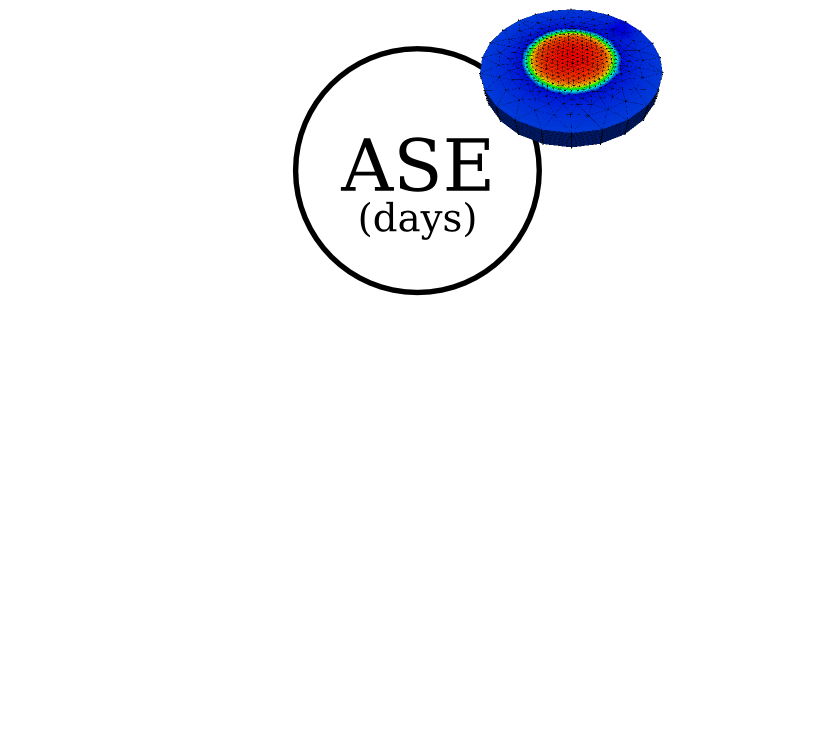
\includegraphics[width=\textwidth]{graphics/ASE_temperature_equilibrium1.png}}
      \myonly{2}{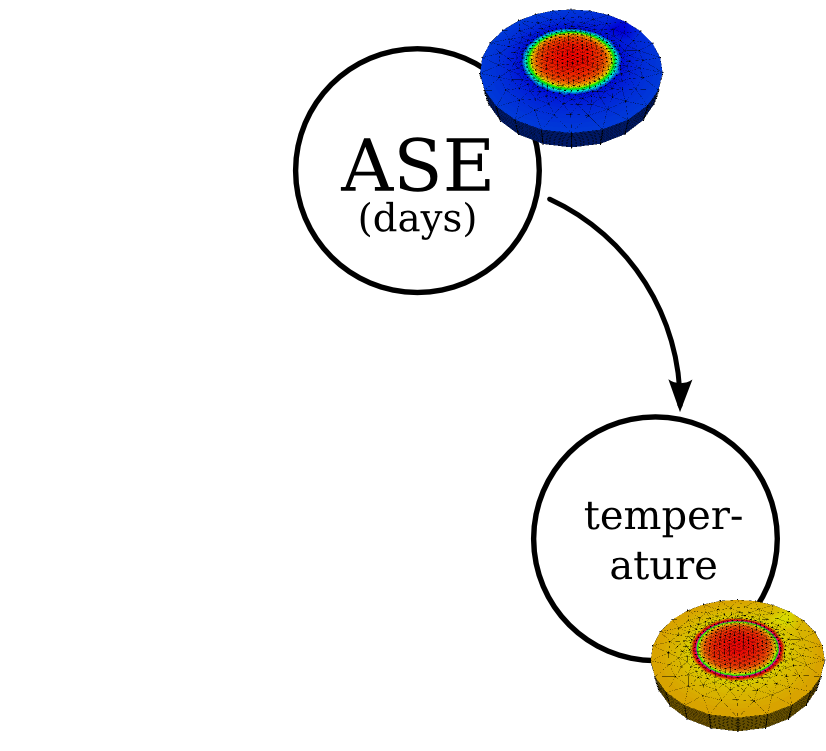
\includegraphics[width=\textwidth]{graphics/ASE_temperature_equilibrium2.png}}
      \myonly{3-4}{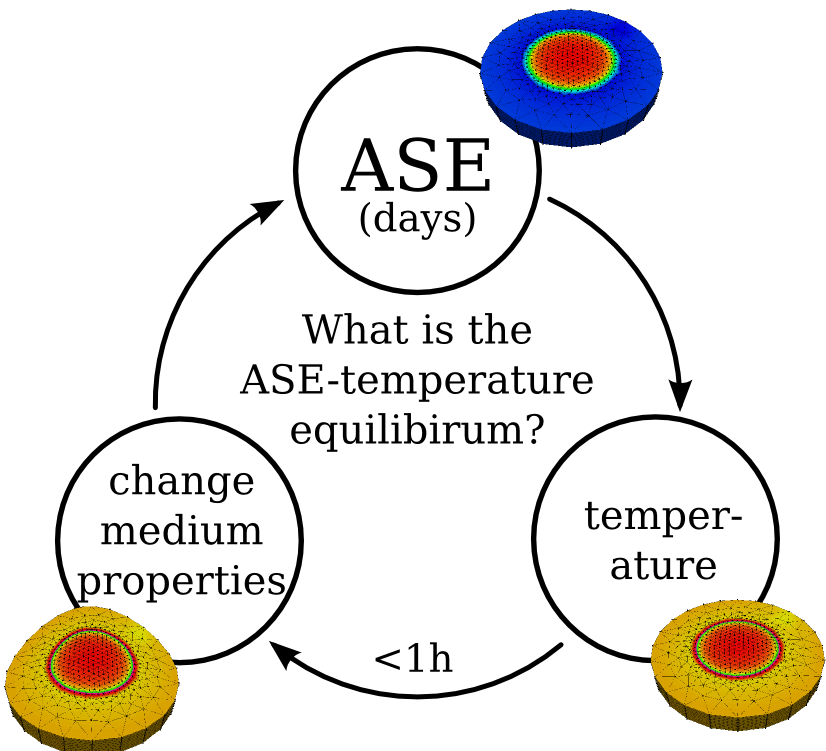
\includegraphics[width=\textwidth]{graphics/ASE_temperature_equilibrium3.png}}
    \end{column}
    \begin{column}{.5\textwidth}
      \begin{itemize}
          \myuncover{2}{4}{
          \item The energy from ASE increases the temperature of the gain medium
          }
          \myuncover{3}{4}{
          \item The change in temperature creates mechanical and optical
            changes, which influence the ASE
          }
          \myuncover{4}{4}{
          \item The calculation of ASE is time-consuming, making an iterative
            computation very costly
          }
      \end{itemize}
    \end{column}

  \end{columns}
\end{frame}

\autobookmark
\begin{frame}[t]{Monte Carlo is an embarrassingly parallel algorithm}
  \myonly{1}{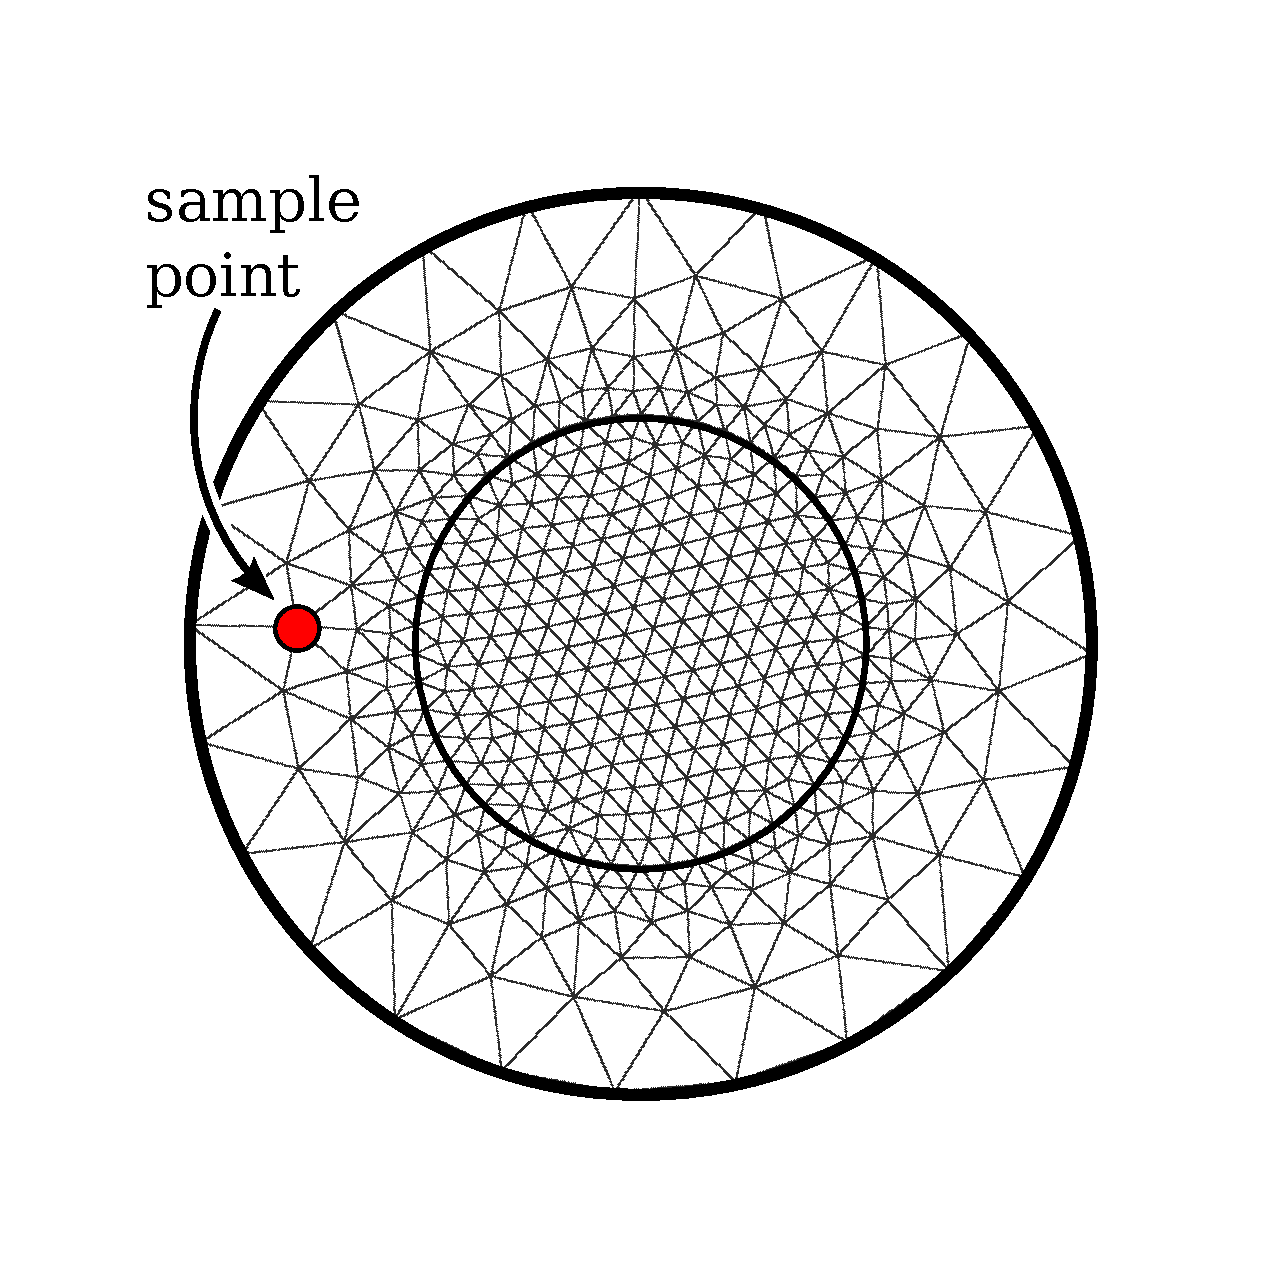
\includegraphics[height=0.6\paperheight]{graphics/monte_carlo_description_0.pdf}}
  \myonly{2}{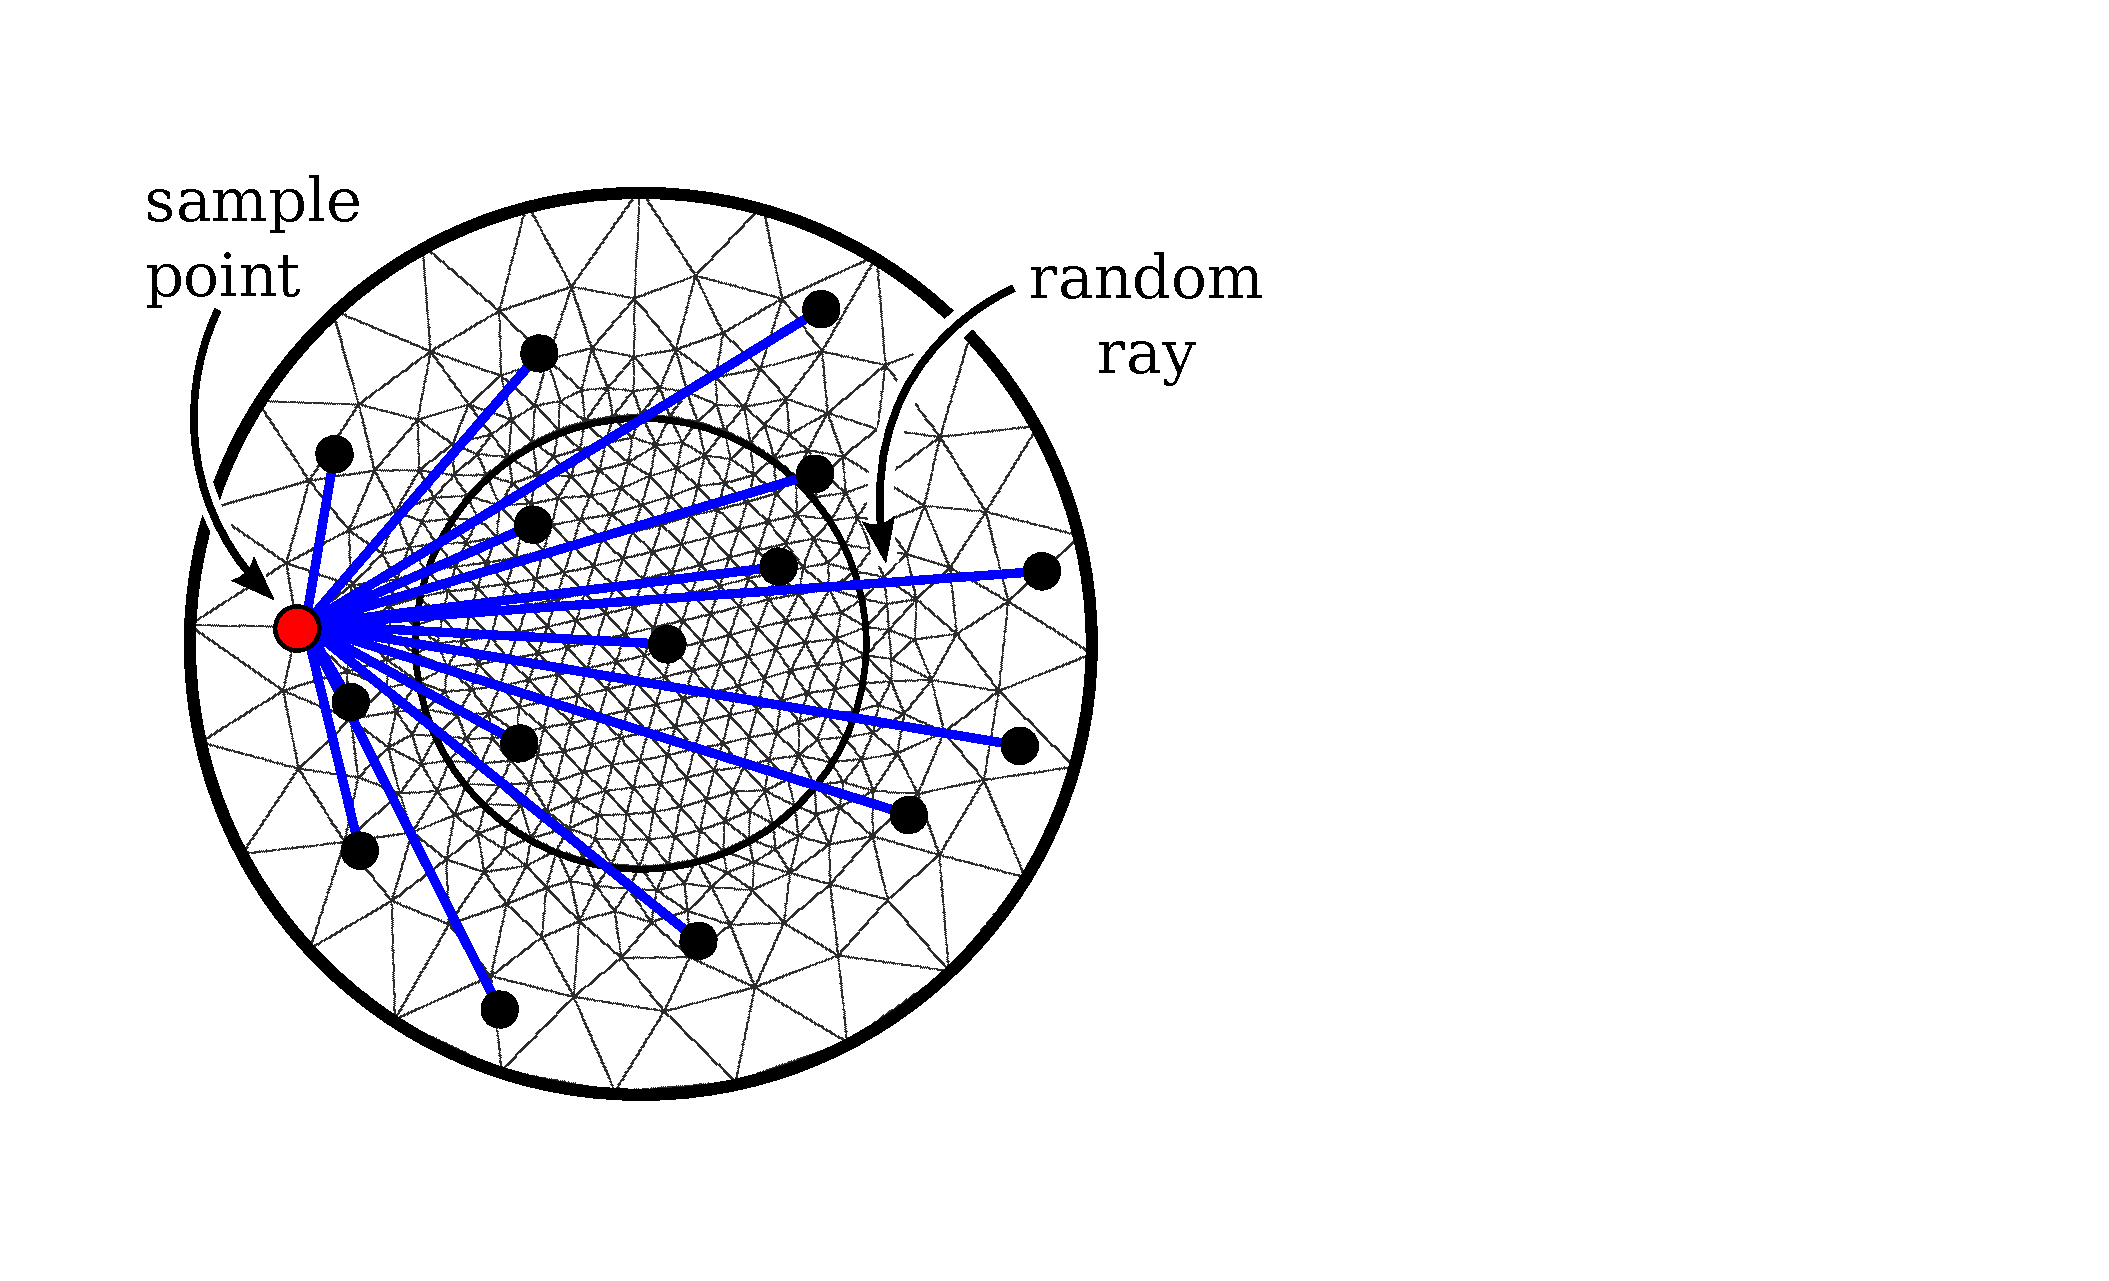
\includegraphics[height=0.6\paperheight]{graphics/monte_carlo_description_1.pdf}}
  %\myonly{3}{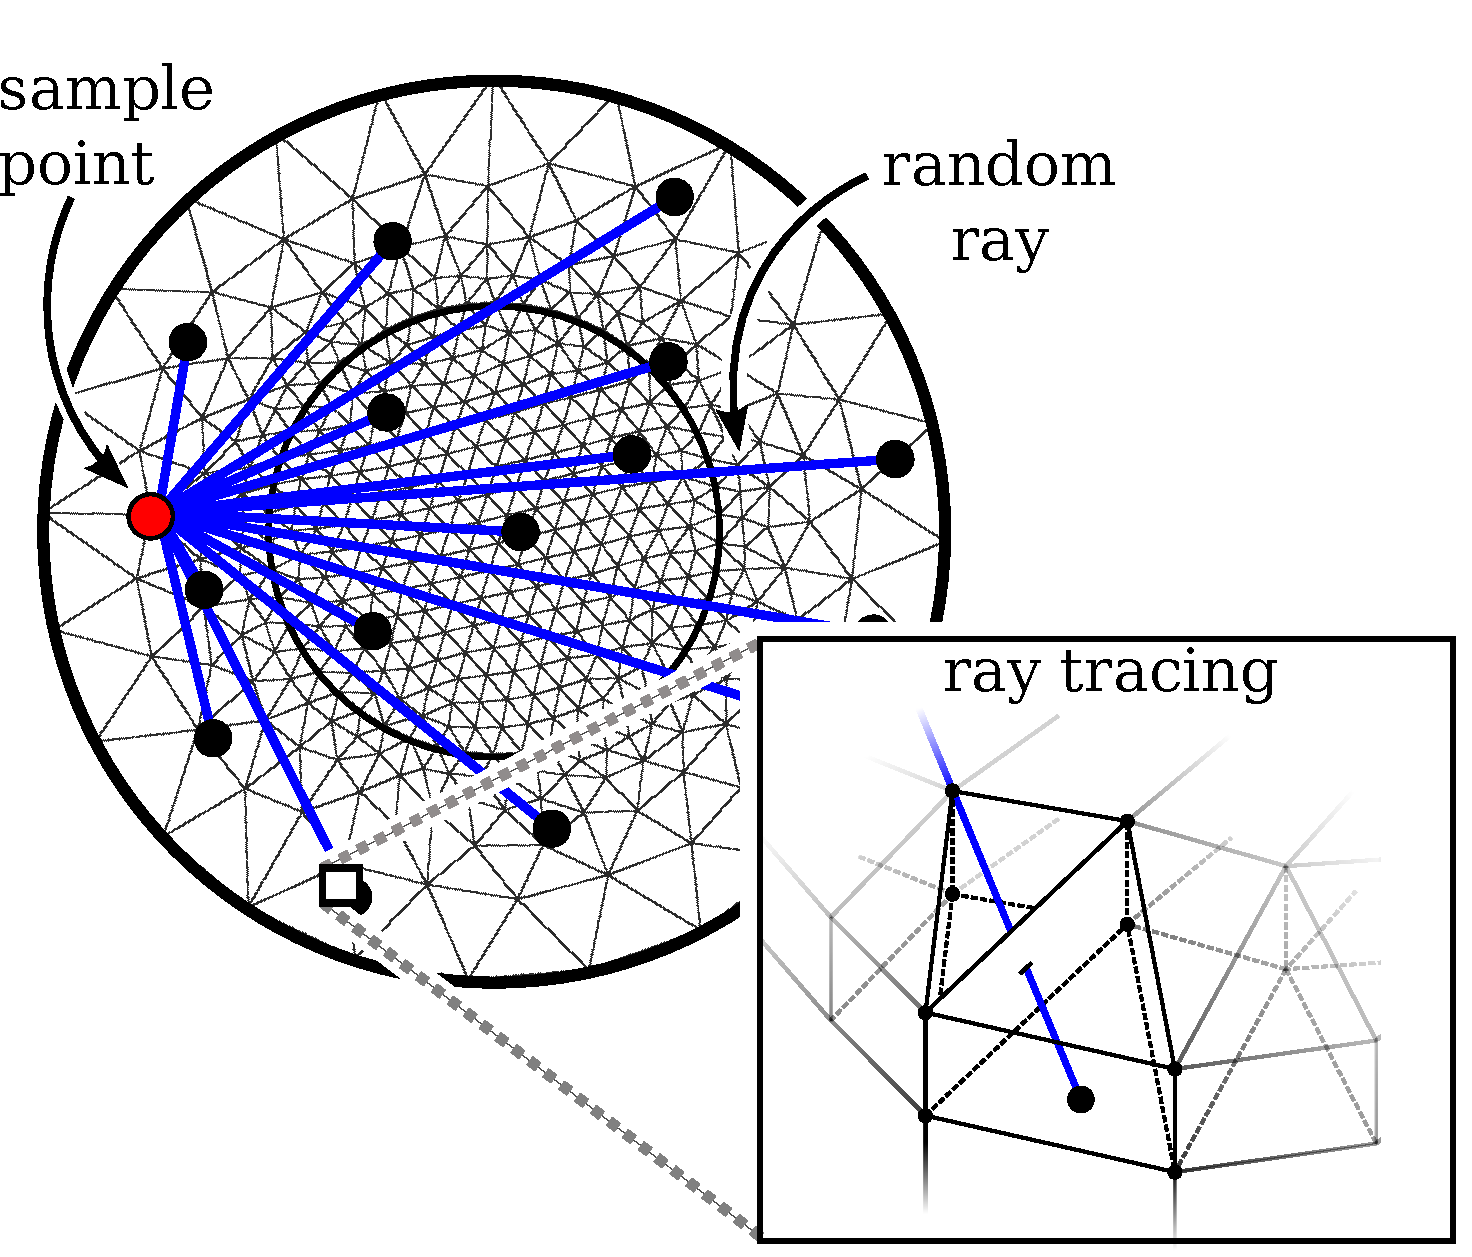
\includegraphics[height=0.6\paperheight]{graphics/monte_carlo_description_2.pdf}}
  %\myonly{4}{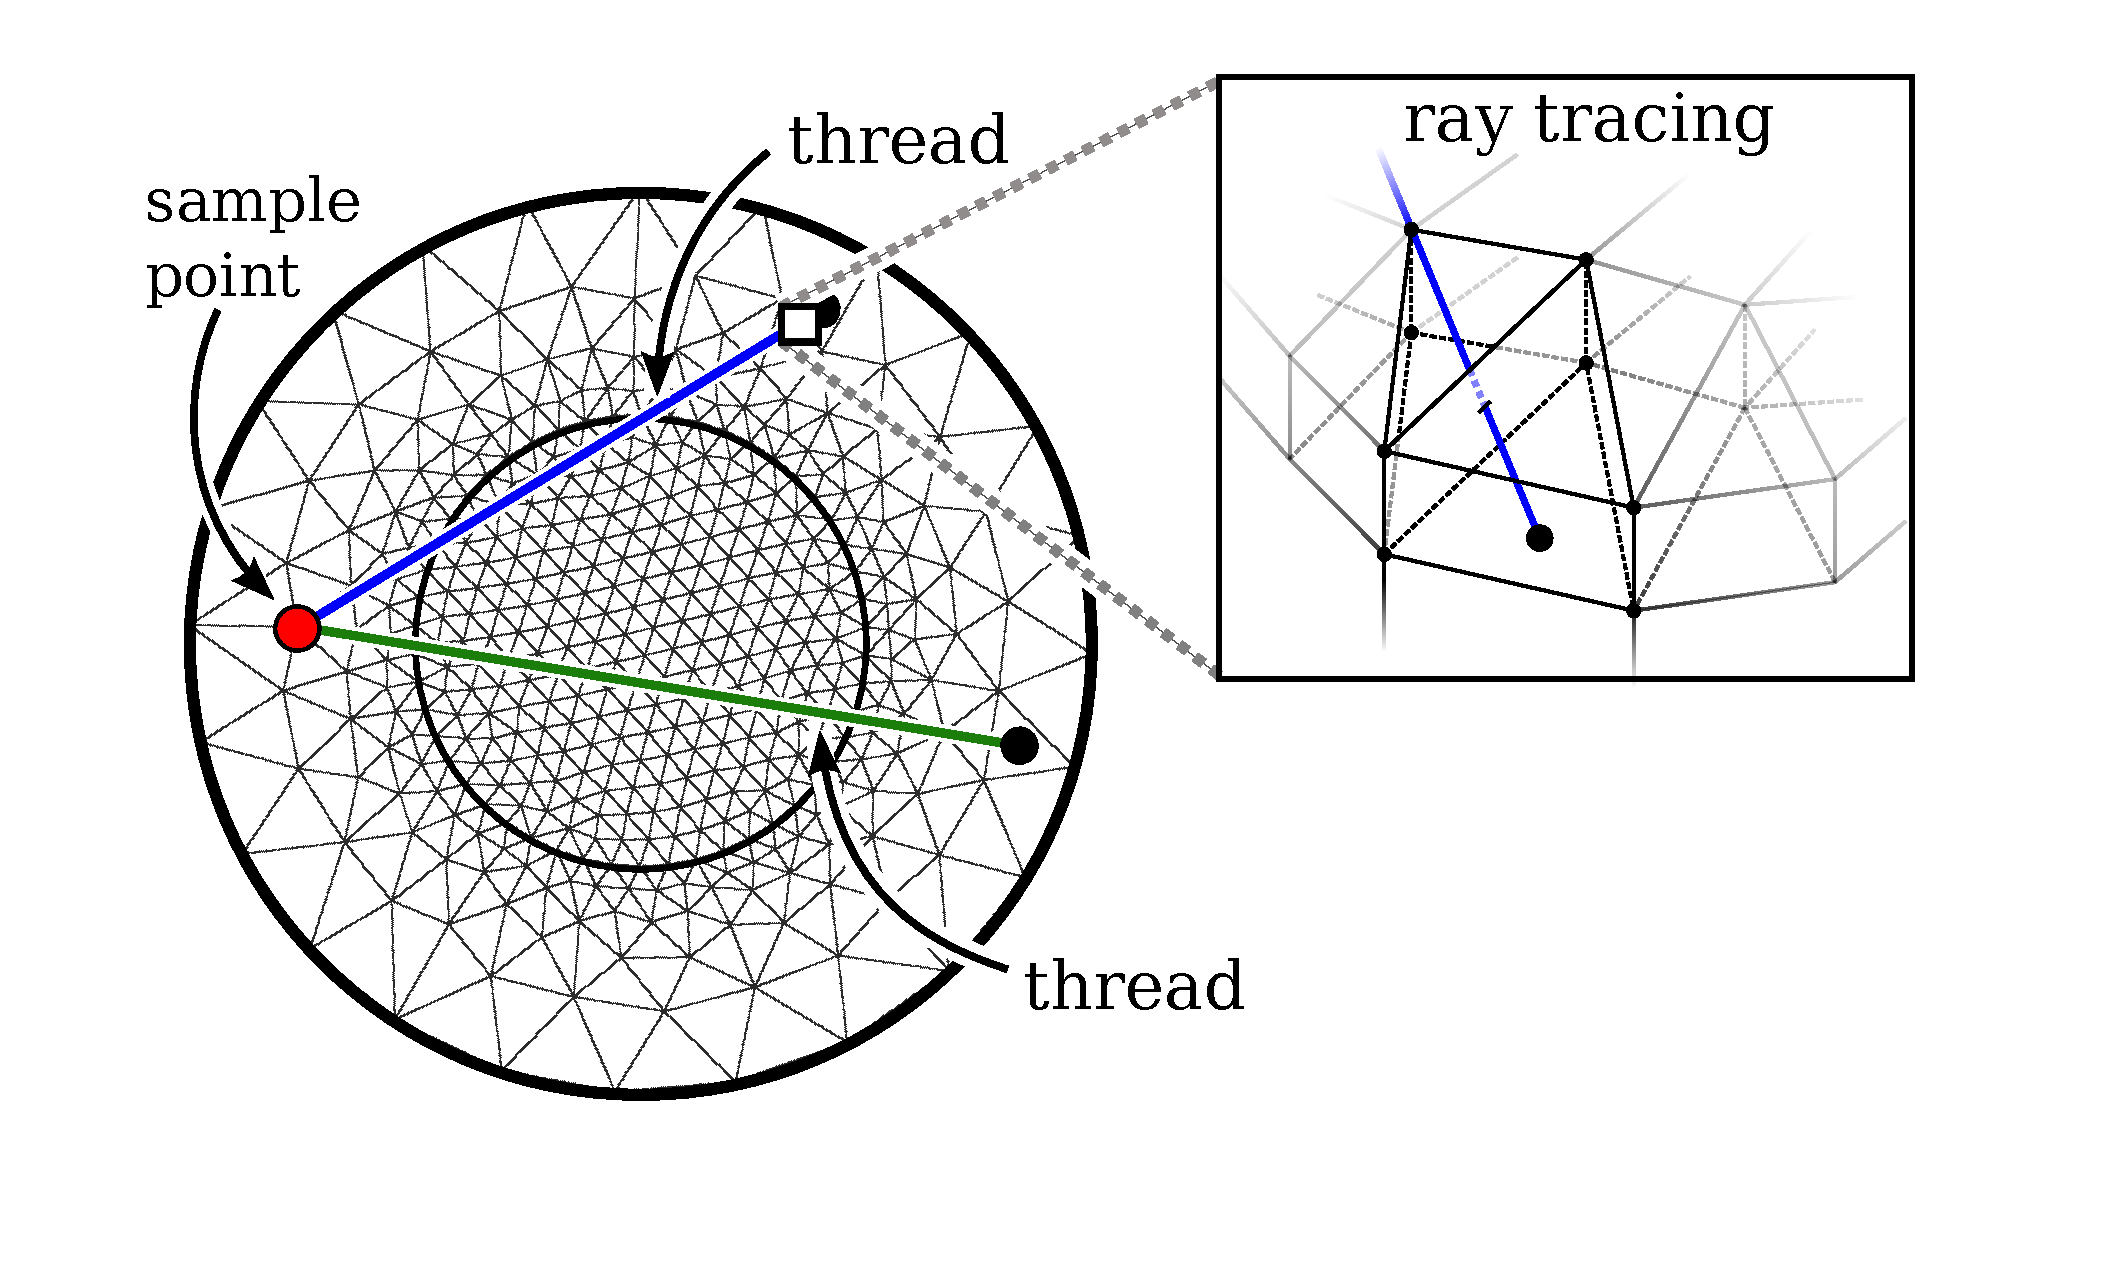
\includegraphics[height=0.6\paperheight]{graphics/monte_carlo_description_3.pdf}}
%
%  \begin{columns}[T]
%
%    \begin{column}{.5\textwidth}
%      \textbf{graphic: ASE crystal, with a photon travelling through it?}\\[2ex]
%      \textbf{alternative: laser setup, pumping a gain medium?}
%    \end{column}
%
%    \begin{column}{.5\textwidth}
%      \begin{itemize}
%      \myuncover{1}{3}{
%        \item In laser physics, gain media are pumped by lasers\\[1ex]
%      }
%      \myuncover{2}{3}{
%        \item Over time, electrons fall back into lower energy levels, causing
%          the spontaneous emission of a photon\\[1ex]
%      }
%      \myuncover{3}{3}{
%        \item Photon travels through the medium, where it is amplified by more
%          photons that are released
%      }
%  \end{itemize}
%    \end{column}
%
%  \end{columns}
\end{frame}

\autobookmark
\begin{frame}[t]{Monte Carlo integration is embarrasingly parallel}
  \begin{columns}[T]
    \begin{column}{.5\textwidth}
      \myonly{1-2}{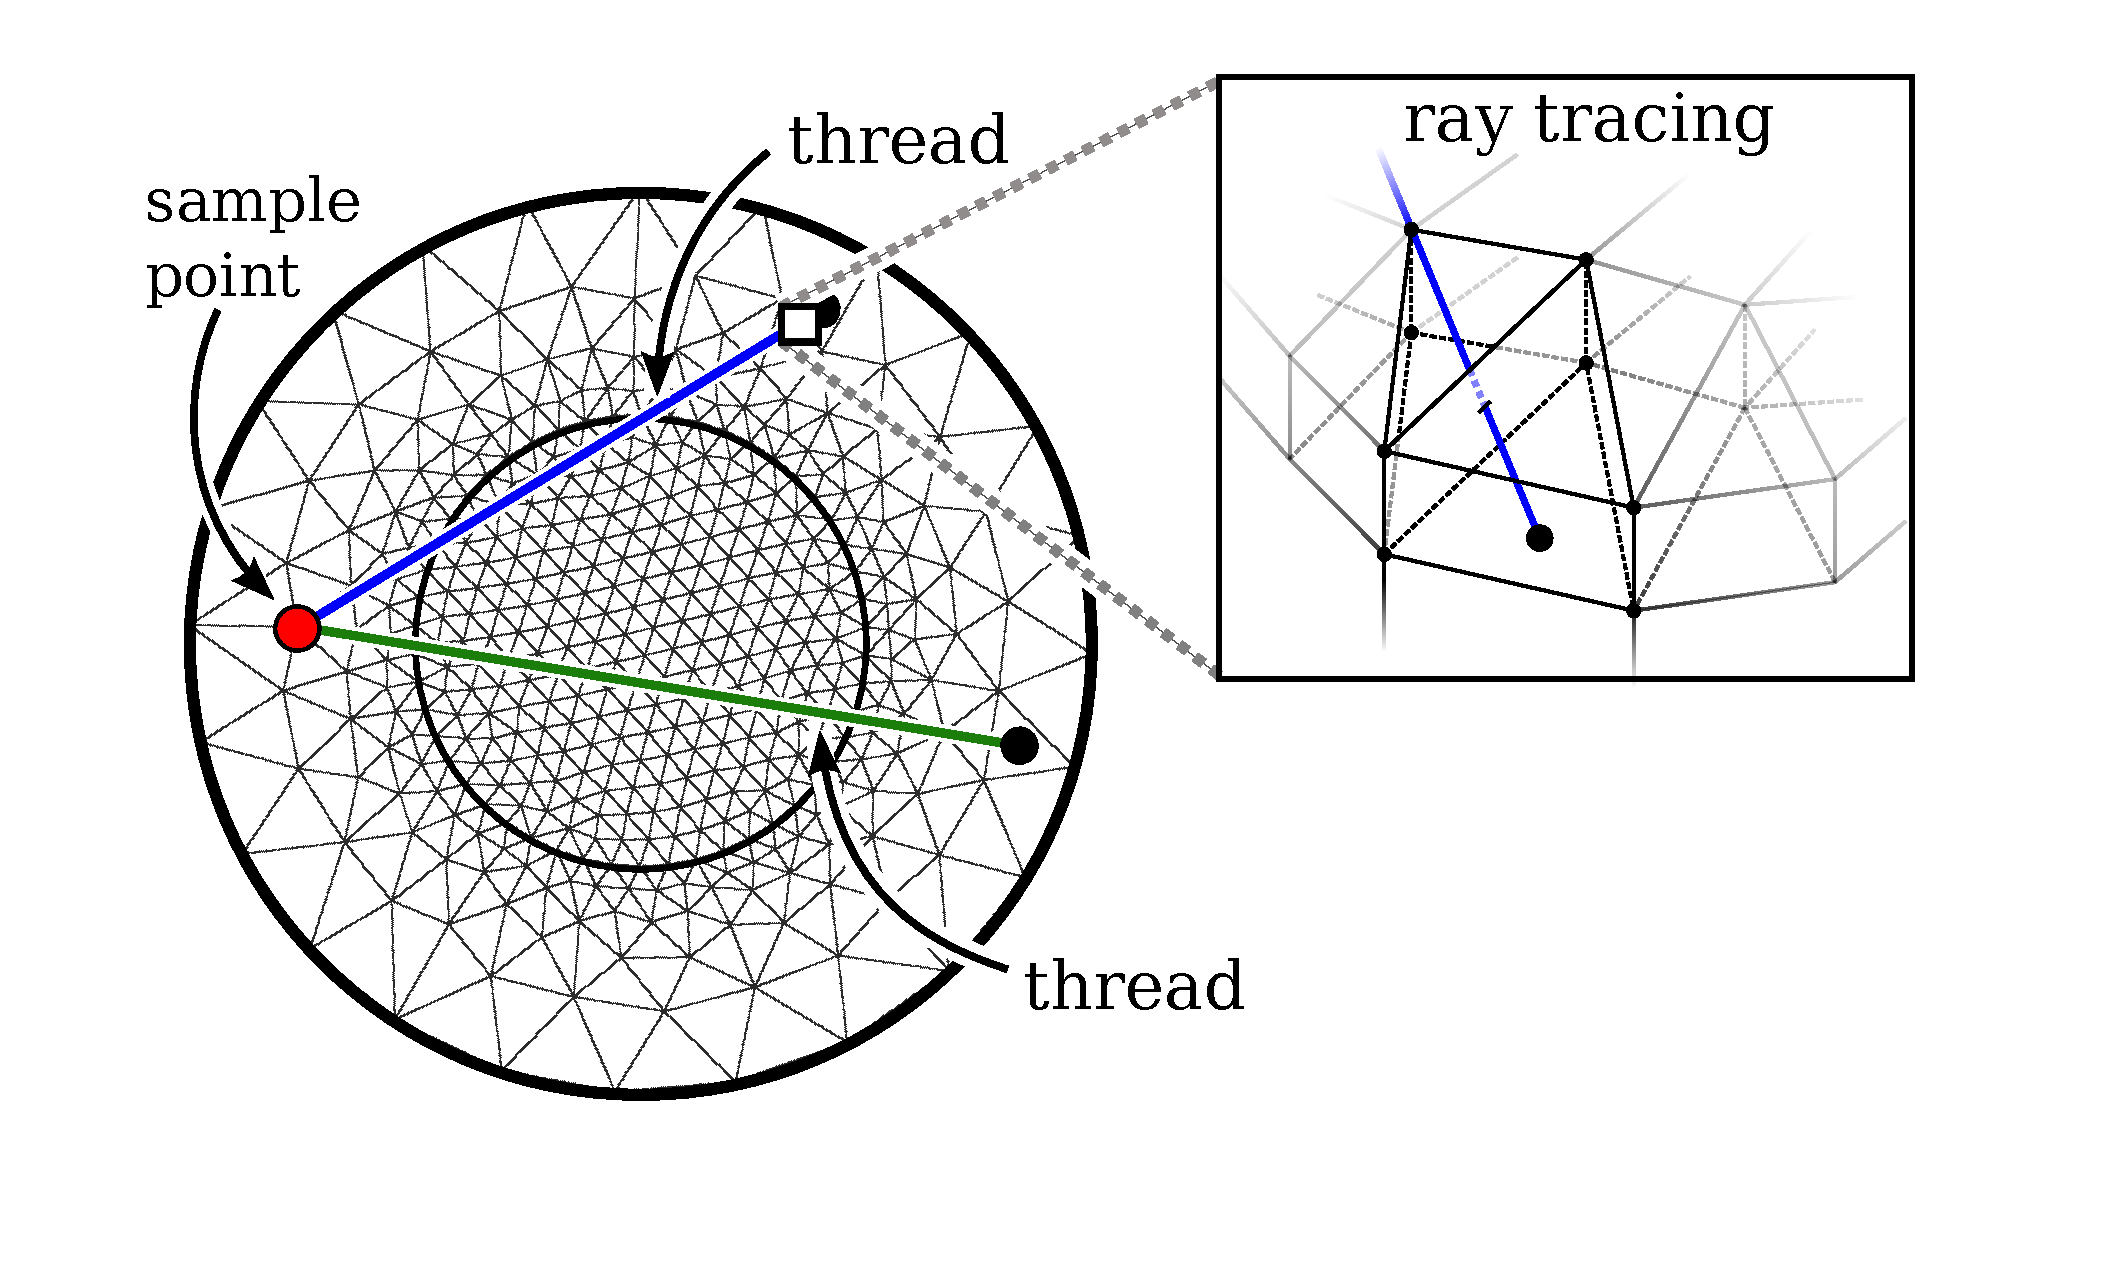
\includegraphics[height=0.55\paperheight]{graphics/monte_carlo_description_3.pdf}}
      \myonly{3-}{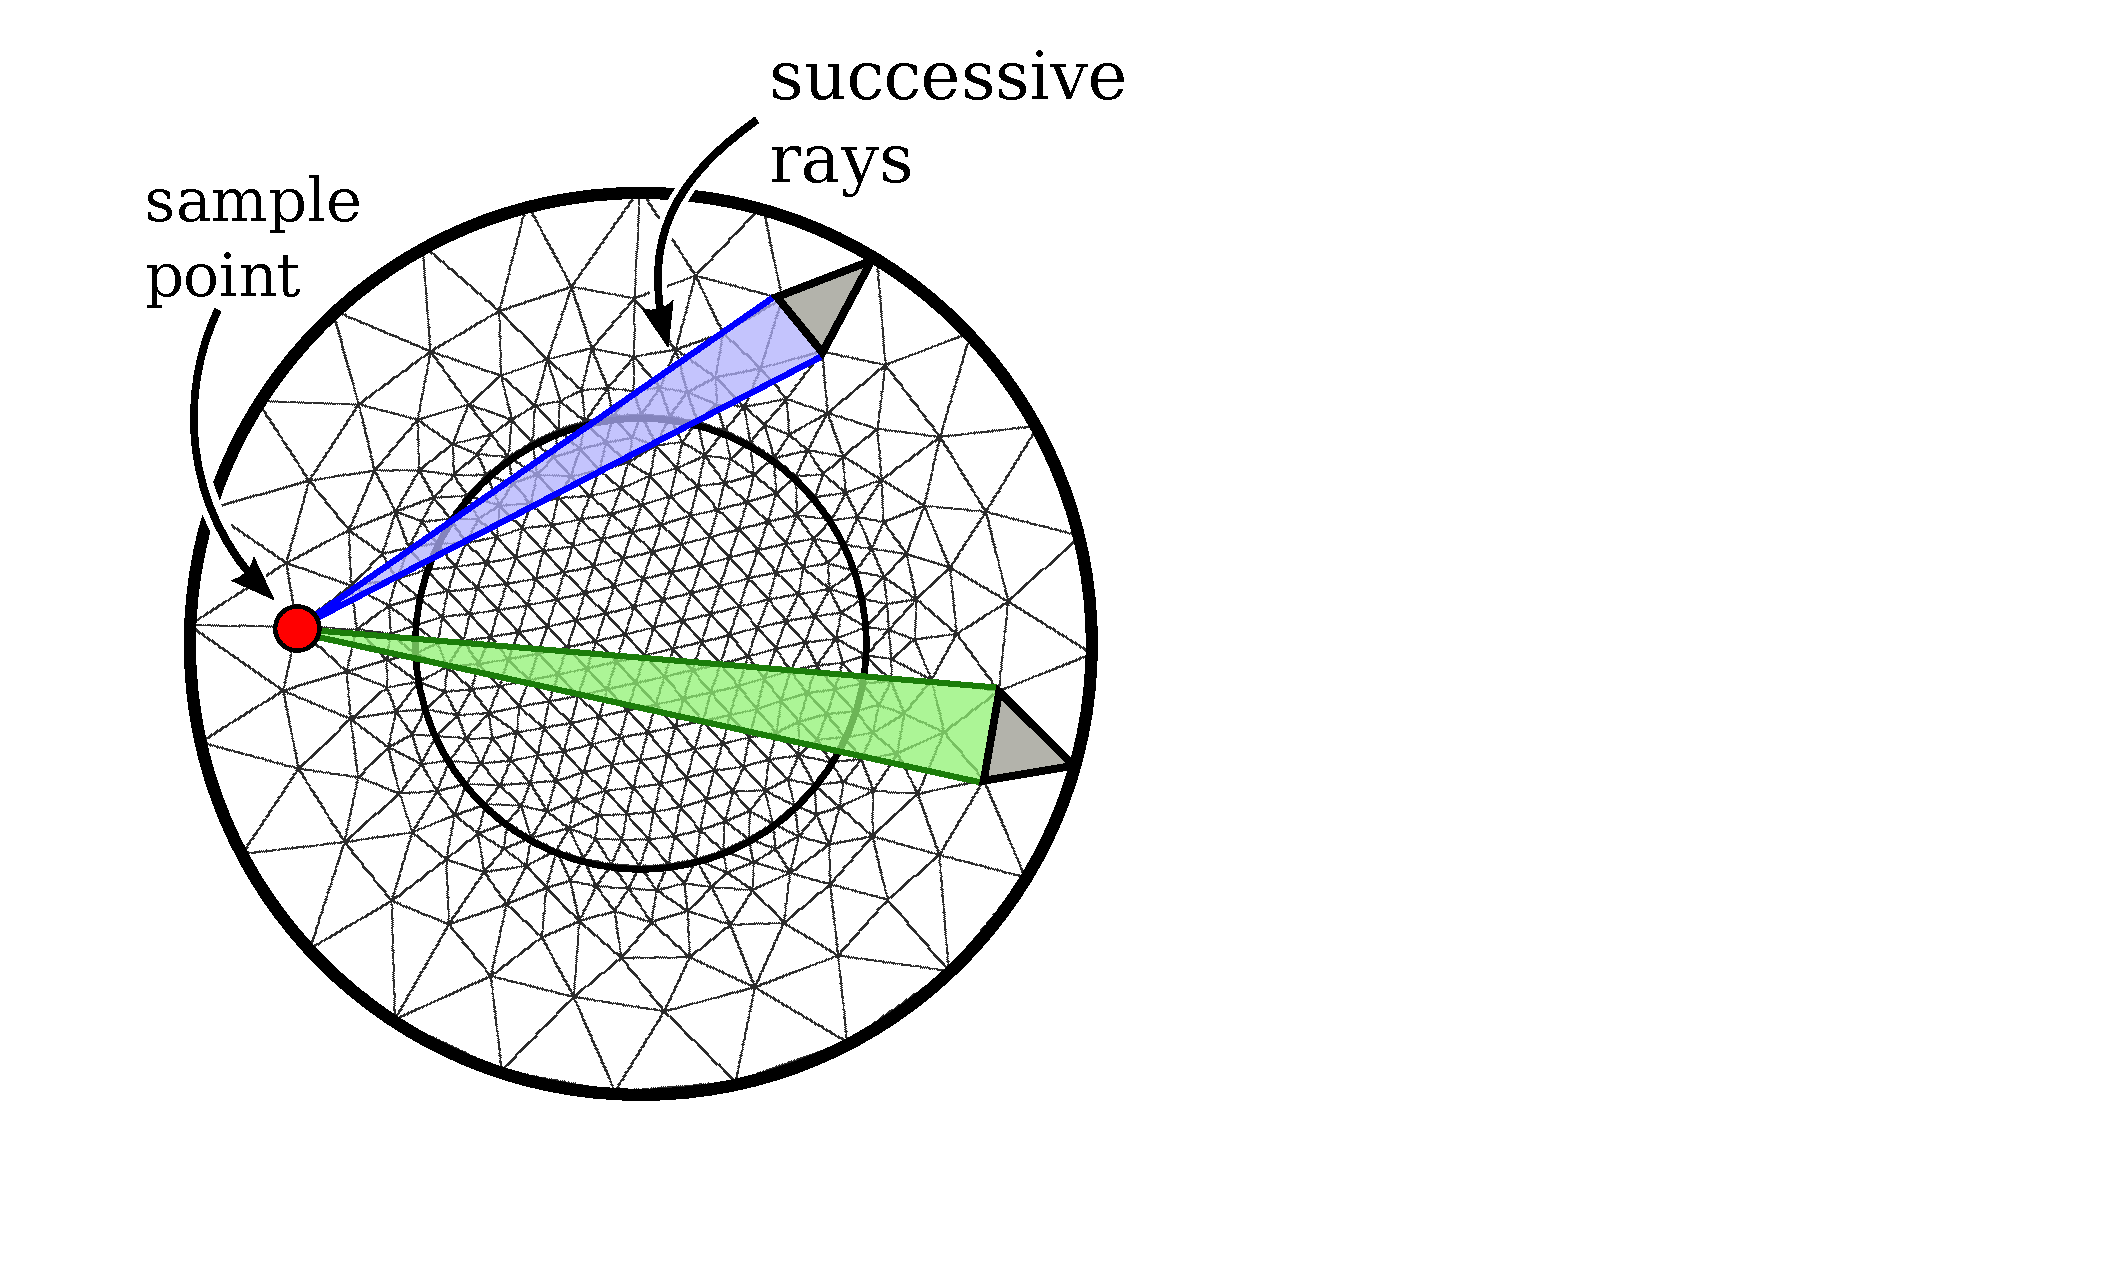
\includegraphics[height=0.55\paperheight]{graphics/monte_carlo_description_4.pdf}}
    \end{column}
    \begin{column}{.5\textwidth}
      \begin{itemize}
        \myuncover{1}{3}{
          \item Each photon is independent from the others
          \item Perfect scenario for accelerators (CUDA)
        }
        \myuncover{2}{3}{
          \item Each thread computes the amplification of a single ray
        }
        \myuncover{3}{3}{
          \item Successive threads start their rays in similar locations
        }
      \end{itemize}
    \end{column}
  \end{columns}
\end{frame}

\autobookmark
\begin{frame}{Using Monte Carlo to simulate ASE}
  \begin{columns}[T]

    \begin{column}{.5\textwidth}
      \textbf{graphic: meshed gain medium}
    \end{column}

    \begin{column}{.5\textwidth}
        The medium is sampled
    \end{column}

  \end{columns}

  \begin{itemize}
      \myuncover{2}{4}{
      \item
        ASE for one of the sample points can be determined:
        \begin{equation}
          \Phi_{ASE}(s_i)=\frac{1}{4\pi}\iint\limits_{V \lambda}
          \frac
          {\hat{n}(r)}
          {\tau_{f}|\rho(r,s_i)|^2}~g(\lambda)~G_{r\rightarrow
          s_i}~dV d\lambda
        \end{equation}
      }
      \myuncover{3}{4}{
      \item With MC, the problem can be transformed into a sum:
        \begin{equation}
          \Phi_{ASE}(s_i) = 
          \frac{1}{4\pi N\tau_f}
          \sum^{N}{1}_{u=0} \hat{n}(r_{i,u}) \cdot
          gain(\overrightarrow{r_{i,u}s_i})
        \end{equation}
      }
      \myuncover{4}{4}{
        \item This Monte Carlo integration can be solved by ray tracing
      }
  \end{itemize}
\end{frame}

%\begin{frame}{Predefined colours}
%  The template defines a set of colours according to the CD guidelines:\par
%  \begin{itemize}
%      \begin{minipage}[t]{0.5\linewidth}
%      \item \textcolor{hzdr-blue}{Helmholtz Blue}    
%      \item \textcolor{hzdr-orange}{Rossendorf Orange}  
%      \item \textcolor{hzdr-darkblue}{Helmholtz Dark Blue}
%      \item \textcolor{hzdr-gray1}{Gray1}   
%      \item \textcolor{hzdr-gray2}{Gray2}   
%      \item \textcolor{hzdr-gray3}{Gray3}   
%      \item \textcolor{hzdr-struct}{Structure of Matter}  
%      \end{minipage}%
%      \begin{minipage}[t]{0.5\linewidth}
%      \item \textcolor{hzdr-health}{Health}  
%      \item \textcolor{hzdr-energy}{Energy}  
%      \item \textcolor{hzdr-earth}{Earth and Environment}   
%      \item \textcolor{hzdr-keytec}{Key Technologies}  
%      \item \textcolor{hzdr-aero}{Aeronautics, Space and Transport}
%      \end{minipage}
%  \end{itemize}
%\end{frame}


\autobookmark
\begin{frame}{Monte Carlo ray tracing is fast on GPGPUs}
  \begin{columns}[T]

    \begin{column}{.7\textwidth}
      \begin{itemize}
          \myuncover{1}{3}{
          \item Because the elements in Monte Carlo are independent, they are
            great to be used with accelerators
          }
          \myuncover{2}{3}{
          \item We used CUDA to improve an exisiting sequential ASE code that
            used MC and ray tracing
          }
          \myuncover{3}{3}{
          \item The calculation can be distributed even more, to utilize a whole
            CPU cluster, which allows to solve huge simulations fast.
          }
      \end{itemize}
    \end{column}

    \begin{column}{.3\textwidth}
      
\includegraphics[height=0.3\paperheight]{graphics/ccoe_small.png}
    \end{column}

  \end{columns}

\end{frame}

%\begin{frame}{Predefined colours}
%  The template defines a set of colours according to the CD guidelines:\par
%  \begin{itemize}
%      \begin{minipage}[t]{0.5\linewidth}
%      \item \textcolor{hzdr-blue}{Helmholtz Blue}    
%      \item \textcolor{hzdr-orange}{Rossendorf Orange}  
%      \item \textcolor{hzdr-darkblue}{Helmholtz Dark Blue}
%      \item \textcolor{hzdr-gray1}{Gray1}   
%      \item \textcolor{hzdr-gray2}{Gray2}   
%      \item \textcolor{hzdr-gray3}{Gray3}   
%      \item \textcolor{hzdr-struct}{Structure of Matter}  
%      \end{minipage}%
%      \begin{minipage}[t]{0.5\linewidth}
%      \item \textcolor{hzdr-health}{Health}  
%      \item \textcolor{hzdr-energy}{Energy}  
%      \item \textcolor{hzdr-earth}{Earth and Environment}   
%      \item \textcolor{hzdr-keytec}{Key Technologies}  
%      \item \textcolor{hzdr-aero}{Aeronautics, Space and Transport}
%      \end{minipage}
%  \end{itemize}
%\end{frame}


\autobookmark
\begin{frame}{Distribution of rays on a GPU}
  \begin{columns}[T]

    \begin{column}{.3\textwidth}
      \textbf{graphic: distribution of threads in a block}
    \end{column}

    \begin{column}{.7\textwidth}
      \begin{itemize}
          \myuncover{1}{4}{
          \item A CUDA thread proceses multiple rays
          \item Reduction over all threads by atomicAdd is the only synchronized part
          }
          \myuncover{2}{4}{
          \item Rays starting in similar positions are grouped together to improve caching
          }
          \myuncover{3}{4}{
          \item Importance sampling distributes rays in the material towards areas of interest
          }
          \myuncover{4}{4}{
          \item Load balancing between blocks, to reduce impact of different ray lengths
          }
      \end{itemize}
    \end{column}


  \end{columns}

\end{frame}

%\begin{frame}{Predefined colours}
%  The template defines a set of colours according to the CD guidelines:\par
%  \begin{itemize}
%      \begin{minipage}[t]{0.5\linewidth}
%      \item \textcolor{hzdr-blue}{Helmholtz Blue}    
%      \item \textcolor{hzdr-orange}{Rossendorf Orange}  
%      \item \textcolor{hzdr-darkblue}{Helmholtz Dark Blue}
%      \item \textcolor{hzdr-gray1}{Gray1}   
%      \item \textcolor{hzdr-gray2}{Gray2}   
%      \item \textcolor{hzdr-gray3}{Gray3}   
%      \item \textcolor{hzdr-struct}{Structure of Matter}  
%      \end{minipage}%
%      \begin{minipage}[t]{0.5\linewidth}
%      \item \textcolor{hzdr-health}{Health}  
%      \item \textcolor{hzdr-energy}{Energy}  
%      \item \textcolor{hzdr-earth}{Earth and Environment}   
%      \item \textcolor{hzdr-keytec}{Key Technologies}  
%      \item \textcolor{hzdr-aero}{Aeronautics, Space and Transport}
%      \end{minipage}
%  \end{itemize}
%\end{frame}


\autobookmark
\begin{frame}{Measuring simulation quality}
  \begin{columns}[T]

    \begin{column}{.3\textwidth}
      \textbf{graphic: delta ASE graphic (mit IS). Or not..}
    \end{column}

    \begin{column}{.7\textwidth}
      \begin{itemize}
          \myuncover{1}{2}{
            \item Using mean squared error to estimate sampling quality
          }
          \myuncover{2}{2}{
            \item Each sample point is independent: each sample point can be optimized individually
          }
      \end{itemize}
    \end{column}


  \end{columns}

\end{frame}

%\begin{frame}{Predefined colours}
%  The template defines a set of colours according to the CD guidelines:\par
%  \begin{itemize}
%      \begin{minipage}[t]{0.5\linewidth}
%      \item \textcolor{hzdr-blue}{Helmholtz Blue}    
%      \item \textcolor{hzdr-orange}{Rossendorf Orange}  
%      \item \textcolor{hzdr-darkblue}{Helmholtz Dark Blue}
%      \item \textcolor{hzdr-gray1}{Gray1}   
%      \item \textcolor{hzdr-gray2}{Gray2}   
%      \item \textcolor{hzdr-gray3}{Gray3}   
%      \item \textcolor{hzdr-struct}{Structure of Matter}  
%      \end{minipage}%
%      \begin{minipage}[t]{0.5\linewidth}
%      \item \textcolor{hzdr-health}{Health}  
%      \item \textcolor{hzdr-energy}{Energy}  
%      \item \textcolor{hzdr-earth}{Earth and Environment}   
%      \item \textcolor{hzdr-keytec}{Key Technologies}  
%      \item \textcolor{hzdr-aero}{Aeronautics, Space and Transport}
%      \end{minipage}
%  \end{itemize}
%\end{frame}


\autobookmark
\begin{frame}[t]{Adaptive sampling to counter high MSE values}
      \myonly{1}{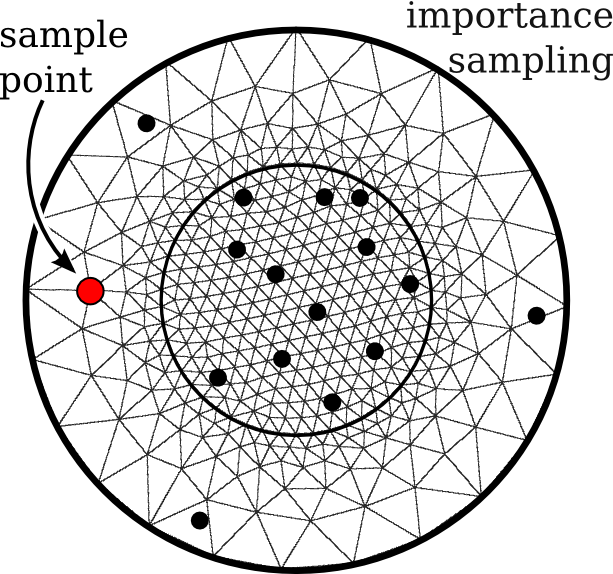
\includegraphics[width=.37\paperwidth]{graphics/ray_distributions3.png}}
      \myonly{2}{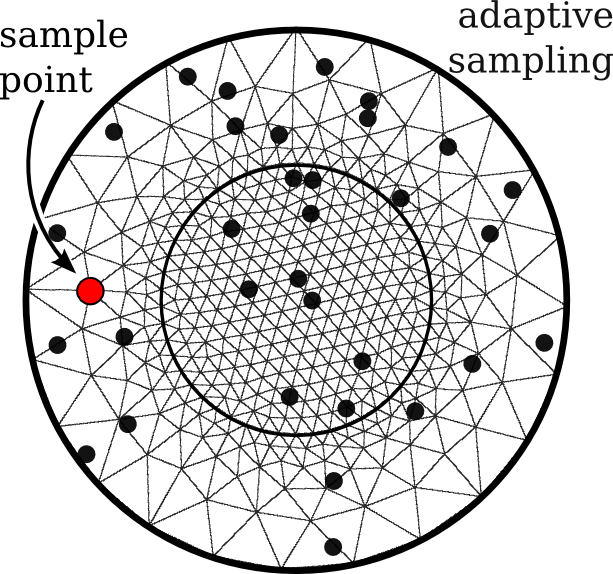
\includegraphics[width=.37\paperwidth]{graphics/ray_distributions4.png}}
      \myonly{1}{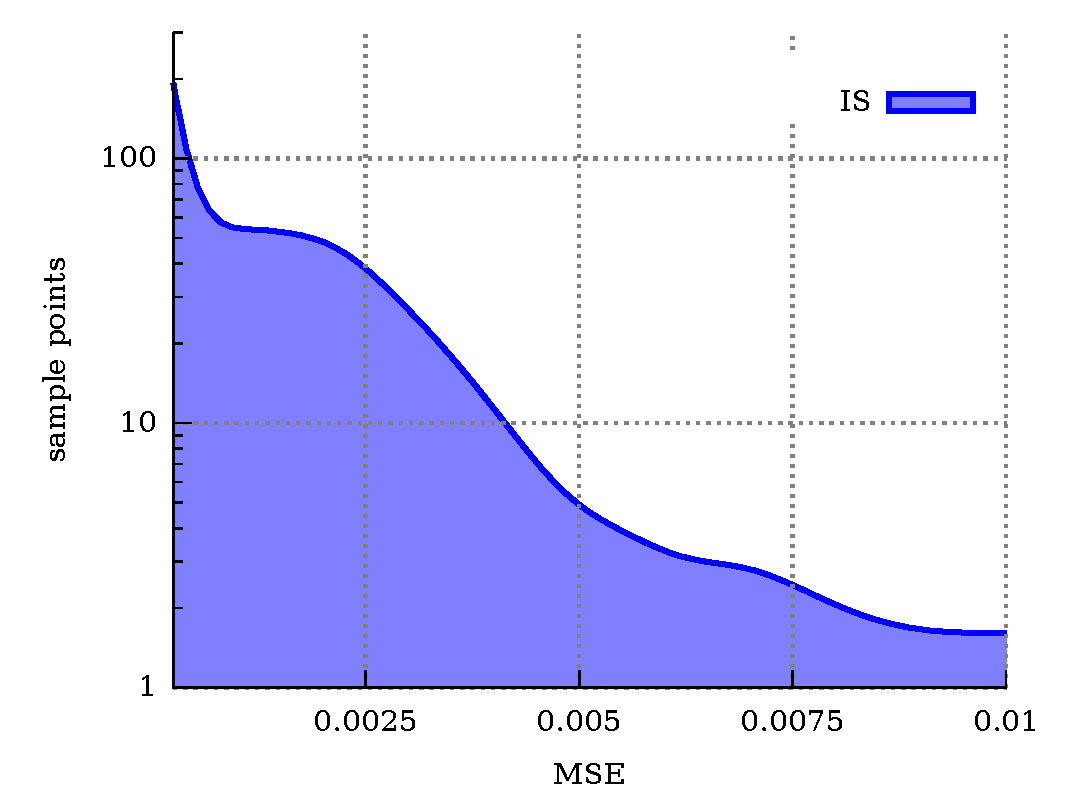
\includegraphics[width=.5\paperwidth]{graphics/mse_histogram_is_as1.pdf}}
      \myonly{2}{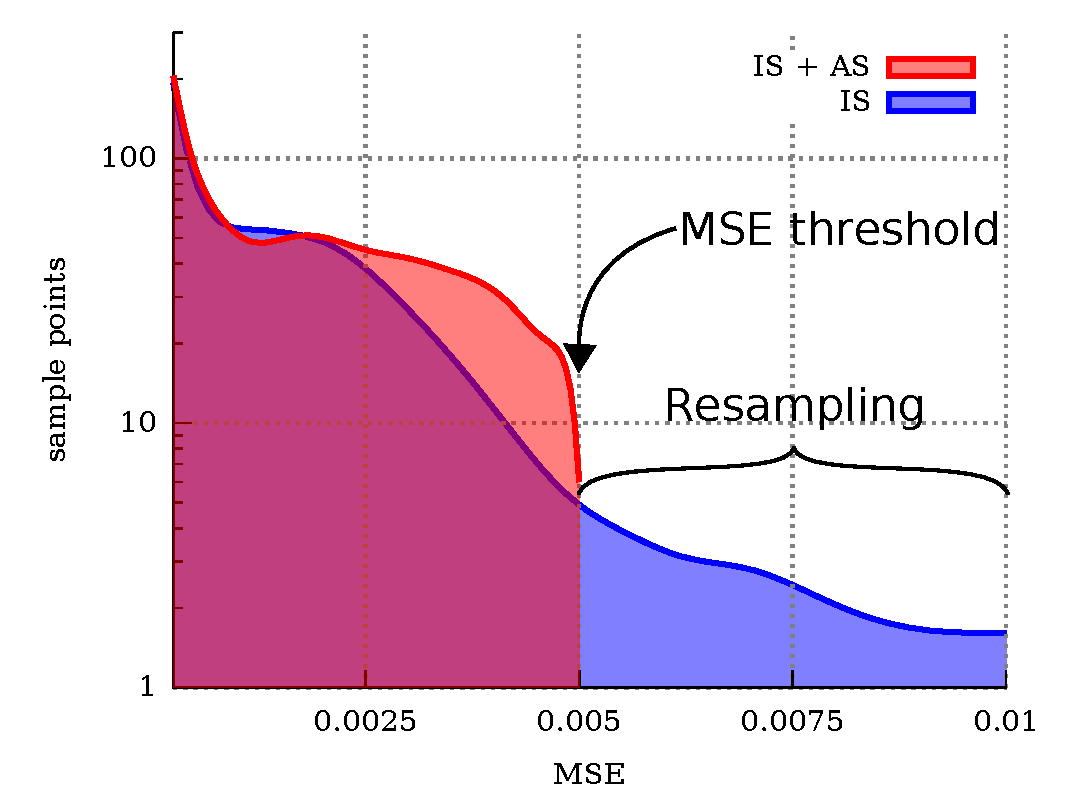
\includegraphics[width=.5\paperwidth]{graphics/mse_histogram_is_as2.pdf}}
      \begin{itemize}
        \myuncover{1}{2}{
        \item Even with importance sampling, high MSE peaks are possible
        }
        \myuncover{2}{2}{
        \item To reach a fixed MSE threshold, the number of rays for the sample point is increased
        }
      \end{itemize}
\end{frame}

\autobookmark
\begin{frame}[t]{Repetetive sampling to counter high MSE values}
      \myonly{1}{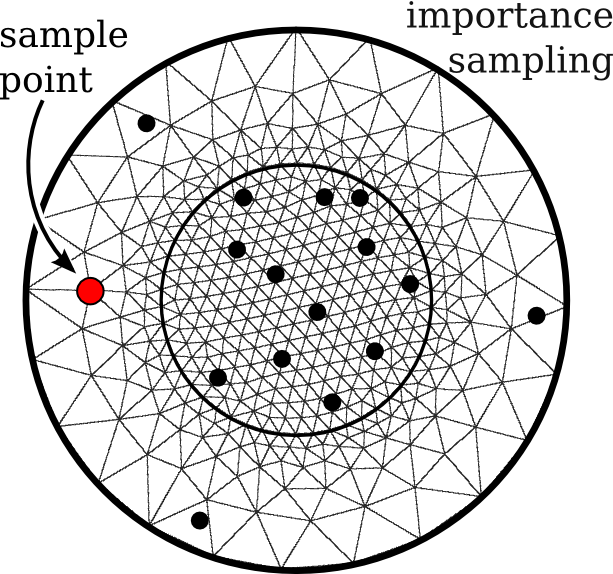
\includegraphics[width=.37\paperwidth]{graphics/ray_distributions3.png}}
      \myonly{2}{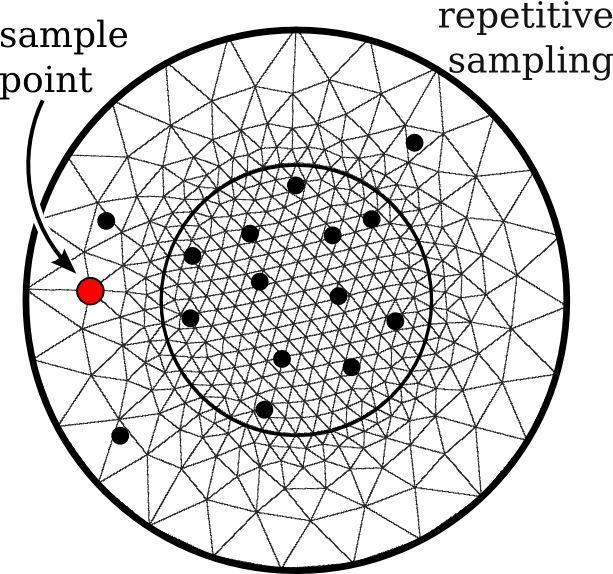
\includegraphics[width=.37\paperwidth]{graphics/ray_distributions5.png}}
      \myonly{1}{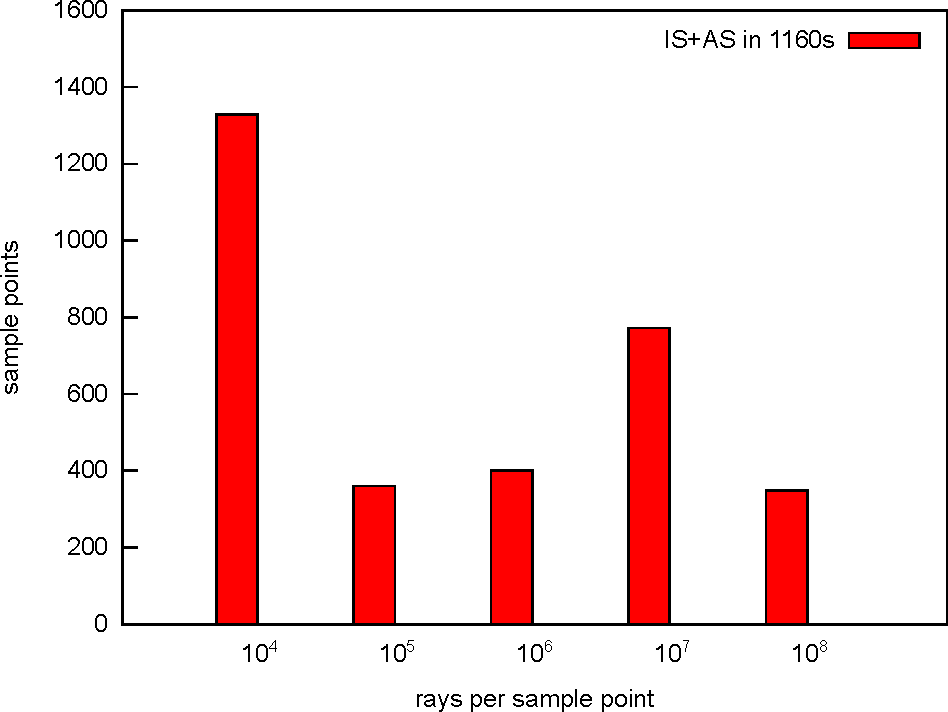
\includegraphics[width=.45\paperwidth]{graphics/mse_histogram_rs1.pdf}}
      \myonly{2}{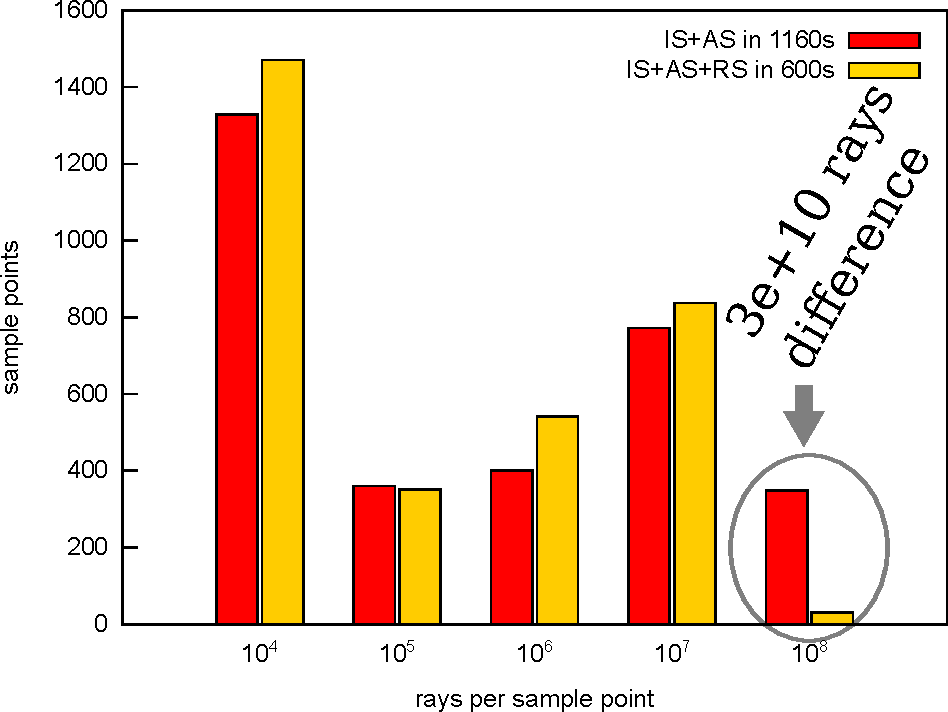
\includegraphics[width=.45\paperwidth]{graphics/mse_histogram_rs2.pdf}}
      \begin{itemize}
          \myuncover{1}{2}{
          \item Sometimes, increasing the number of rays is not necessary, because the high MSE was caused by a really unlucky seed for the PRNG
          }
          \myuncover{2}{2}{
          \item Idea: it might be enough to introduce random restarts, since this is much faster than increasing the number of rays
          }
      \end{itemize}
\end{frame}

%\begin{frame}{Predefined colours}
%  The template defines a set of colours according to the CD guidelines:\par
%  \begin{itemize}
%      \begin{minipage}[t]{0.5\linewidth}
%      \item \textcolor{hzdr-blue}{Helmholtz Blue}    
%      \item \textcolor{hzdr-orange}{Rossendorf Orange}  
%      \item \textcolor{hzdr-darkblue}{Helmholtz Dark Blue}
%      \item \textcolor{hzdr-gray1}{Gray1}   
%      \item \textcolor{hzdr-gray2}{Gray2}   
%      \item \textcolor{hzdr-gray3}{Gray3}   
%      \item \textcolor{hzdr-struct}{Structure of Matter}  
%      \end{minipage}%
%      \begin{minipage}[t]{0.5\linewidth}
%      \item \textcolor{hzdr-health}{Health}  
%      \item \textcolor{hzdr-energy}{Energy}  
%      \item \textcolor{hzdr-earth}{Earth and Environment}   
%      \item \textcolor{hzdr-keytec}{Key Technologies}  
%      \item \textcolor{hzdr-aero}{Aeronautics, Space and Transport}
%      \end{minipage}
%  \end{itemize}
%\end{frame}


\autobookmark
\begin{frame}[t]{Sample points can be distributed in a cluster}
  \begin{columns}[T]

    \begin{column}{.5\textwidth}
      \myonly{2}{
\includegraphics[width=0.5\paperwidth]{graphics/load_balancing_MPI_0.pdf}}
      \myonly{3}{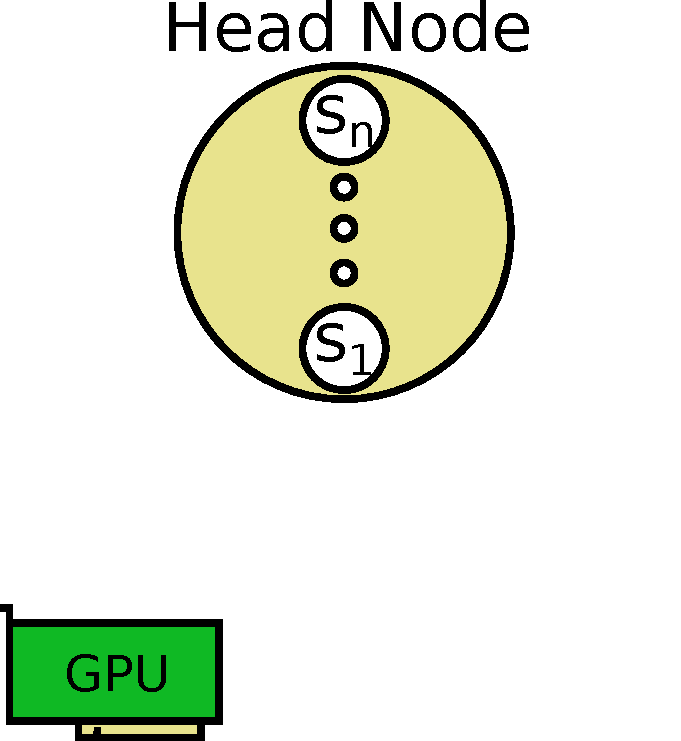
\includegraphics[width=0.5\paperwidth]{graphics/load_balancing_MPI_1.pdf}}
      \myonly{4-5}{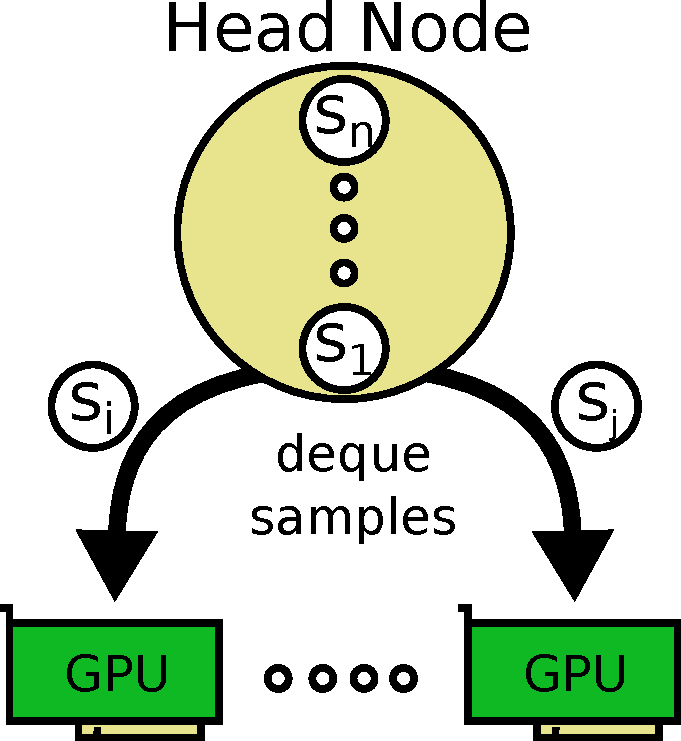
\includegraphics[width=0.5\paperwidth]{graphics/load_balancing_MPI_2.pdf}}
    \end{column}

    \begin{column}{.5\textwidth}
      \begin{itemize}
          \myuncover{1}{5}{
            \item Until now: simulation of a single sample point on a single GPU
            \item All sample points are independent: let's use a cluster for that
          }
          \myuncover{2}{5}{
            \item Each GPU has all the necessary data
            \item MPI is used as communication framework
          }
          \myuncover{3}{5}{
            \item Head node assigns work to the GPU
          }
          \myuncover{4}{5}{
            \item Add more GPUs as needed
          }
          \myuncover{5}{5}{
            \item Load balancing, even when some sample points take longer than others
          }
      \end{itemize}
    \end{column}

  \end{columns}
\end{frame}

%\begin{frame}{Predefined colours}
%  The template defines a set of colours according to the CD guidelines:\par
%  \begin{itemize}
%      \begin{minipage}[t]{0.5\linewidth}
%      \item \textcolor{hzdr-blue}{Helmholtz Blue}    
%      \item \textcolor{hzdr-orange}{Rossendorf Orange}  
%      \item \textcolor{hzdr-darkblue}{Helmholtz Dark Blue}
%      \item \textcolor{hzdr-gray1}{Gray1}   
%      \item \textcolor{hzdr-gray2}{Gray2}   
%      \item \textcolor{hzdr-gray3}{Gray3}   
%      \item \textcolor{hzdr-struct}{Structure of Matter}  
%      \end{minipage}%
%      \begin{minipage}[t]{0.5\linewidth}
%      \item \textcolor{hzdr-health}{Health}  
%      \item \textcolor{hzdr-energy}{Energy}  
%      \item \textcolor{hzdr-earth}{Earth and Environment}   
%      \item \textcolor{hzdr-keytec}{Key Technologies}  
%      \item \textcolor{hzdr-aero}{Aeronautics, Space and Transport}
%      \end{minipage}
%  \end{itemize}
%\end{frame}


\autobookmark
\begin{frame}{Simulation has a strong agreement with experimental data}
  \begin{columns}[T]

    \begin{column}{.5\textwidth}
      \myonly{1}{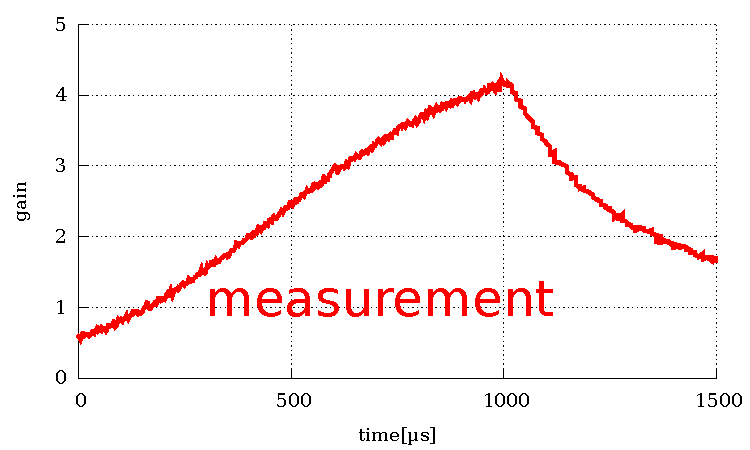
\includegraphics[width=0.5\paperwidth]{graphics/benchmark_results_0.pdf}}
      \myonly{2-}{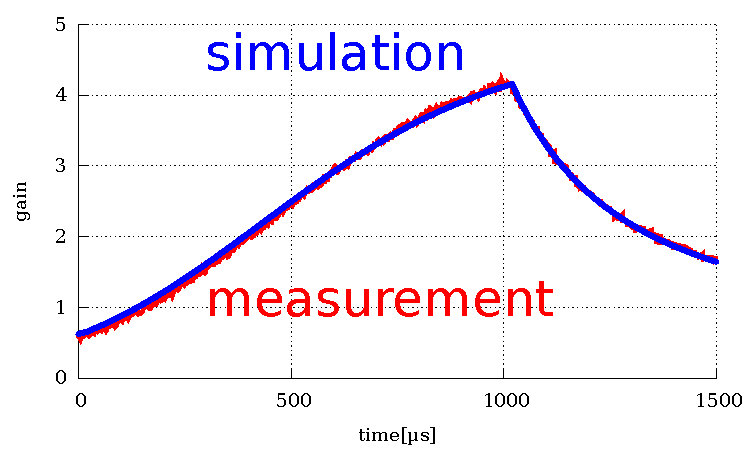
\includegraphics[width=0.5\paperwidth]{graphics/benchmark_results_1.pdf}}
    \end{column}

    \begin{column}{.5\textwidth}
      \begin{itemize}
          \myuncover{1}{3}{
            \item Reminder: plot from experimental data
          }
          \myuncover{2}{3}{
            \item Simulating the experiment gives the following graph, which
              looks almost like a function fit, but isn't
          }
          \myuncover{3}{3}{
            \item Simulation takes about 7h on 1 GPU
          }
      \end{itemize}
    \end{column}

  \end{columns}
\end{frame}

%\begin{frame}{Predefined colours}
%  The template defines a set of colours according to the CD guidelines:\par
%  \begin{itemize}
%      \begin{minipage}[t]{0.5\linewidth}
%      \item \textcolor{hzdr-blue}{Helmholtz Blue}    
%      \item \textcolor{hzdr-orange}{Rossendorf Orange}  
%      \item \textcolor{hzdr-darkblue}{Helmholtz Dark Blue}
%      \item \textcolor{hzdr-gray1}{Gray1}   
%      \item \textcolor{hzdr-gray2}{Gray2}   
%      \item \textcolor{hzdr-gray3}{Gray3}   
%      \item \textcolor{hzdr-struct}{Structure of Matter}  
%      \end{minipage}%
%      \begin{minipage}[t]{0.5\linewidth}
%      \item \textcolor{hzdr-health}{Health}  
%      \item \textcolor{hzdr-energy}{Energy}  
%      \item \textcolor{hzdr-earth}{Earth and Environment}   
%      \item \textcolor{hzdr-keytec}{Key Technologies}  
%      \item \textcolor{hzdr-aero}{Aeronautics, Space and Transport}
%      \end{minipage}
%  \end{itemize}
%\end{frame}


\autobookmark
\begin{frame}{Simulation has a strong agreement with experimental data}
  \begin{columns}[T]

    \begin{column}{.5\textwidth}
      \myonly{1}{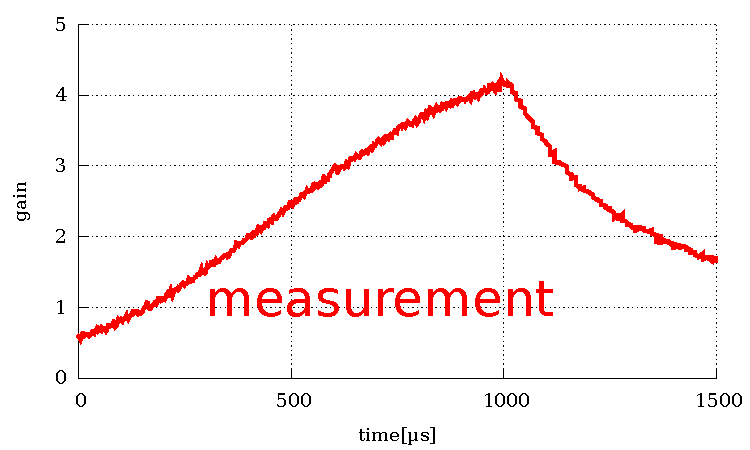
\includegraphics[width=0.5\paperwidth]{graphics/benchmark_results_0.pdf}}
      \myonly{2-}{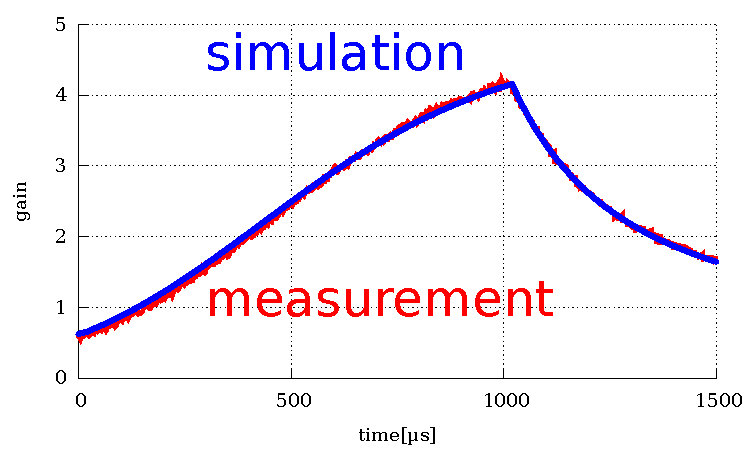
\includegraphics[width=0.5\paperwidth]{graphics/benchmark_results_1.pdf}}
    \end{column}

    \begin{column}{.5\textwidth}
      \begin{itemize}
          \myuncover{1}{3}{
            \item Reminder: plot from experimental data
          }
          \myuncover{2}{3}{
            \item Simulating the experiment gives the following graph, which
              looks almost like a function fit, but isn't
          }
          \myuncover{3}{3}{
            \item Simulation takes about 7h on 1 GPU
          }
      \end{itemize}
    \end{column}

  \end{columns}
\end{frame}

%\begin{frame}{Predefined colours}
%  The template defines a set of colours according to the CD guidelines:\par
%  \begin{itemize}
%      \begin{minipage}[t]{0.5\linewidth}
%      \item \textcolor{hzdr-blue}{Helmholtz Blue}    
%      \item \textcolor{hzdr-orange}{Rossendorf Orange}  
%      \item \textcolor{hzdr-darkblue}{Helmholtz Dark Blue}
%      \item \textcolor{hzdr-gray1}{Gray1}   
%      \item \textcolor{hzdr-gray2}{Gray2}   
%      \item \textcolor{hzdr-gray3}{Gray3}   
%      \item \textcolor{hzdr-struct}{Structure of Matter}  
%      \end{minipage}%
%      \begin{minipage}[t]{0.5\linewidth}
%      \item \textcolor{hzdr-health}{Health}  
%      \item \textcolor{hzdr-energy}{Energy}  
%      \item \textcolor{hzdr-earth}{Earth and Environment}   
%      \item \textcolor{hzdr-keytec}{Key Technologies}  
%      \item \textcolor{hzdr-aero}{Aeronautics, Space and Transport}
%      \end{minipage}
%  \end{itemize}
%\end{frame}


\autobookmark
\begin{frame}{Huge speedup compared to CPU implementation}
  \begin{columns}[T]

    \begin{column}{.5\textwidth}
    \myuncover{1}{2}{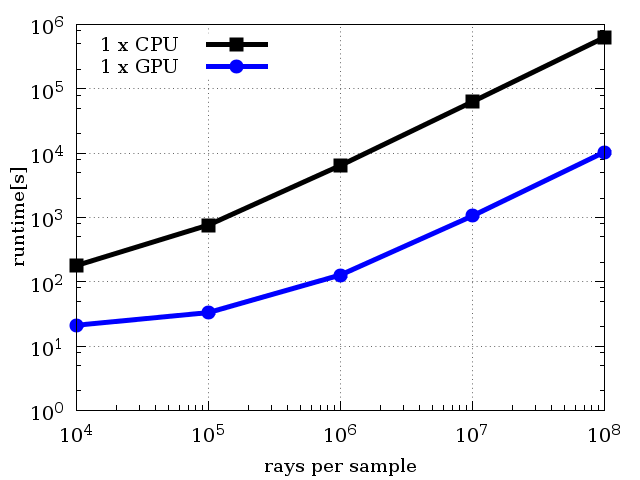
\includegraphics[width=0.5\paperwidth]{graphics/runtime.png}}
    \end{column}

    \begin{column}{.5\textwidth}
      \begin{itemize}
          \myuncover{1}{2}{
            \item Speedup of 2 orders of magnitude
          }
          \myuncover{2}{2}{
            \item Performing the previous simulation on a CPU would take about 1 month
            \item Way too long for larger gain media
          }
      \end{itemize}
    \end{column}

  \end{columns}
\end{frame}

%\begin{frame}{Predefined colours}
%  The template defines a set of colours according to the CD guidelines:\par
%  \begin{itemize}
%      \begin{minipage}[t]{0.5\linewidth}
%      \item \textcolor{hzdr-blue}{Helmholtz Blue}    
%      \item \textcolor{hzdr-orange}{Rossendorf Orange}  
%      \item \textcolor{hzdr-darkblue}{Helmholtz Dark Blue}
%      \item \textcolor{hzdr-gray1}{Gray1}   
%      \item \textcolor{hzdr-gray2}{Gray2}   
%      \item \textcolor{hzdr-gray3}{Gray3}   
%      \item \textcolor{hzdr-struct}{Structure of Matter}  
%      \end{minipage}%
%      \begin{minipage}[t]{0.5\linewidth}
%      \item \textcolor{hzdr-health}{Health}  
%      \item \textcolor{hzdr-energy}{Energy}  
%      \item \textcolor{hzdr-earth}{Earth and Environment}   
%      \item \textcolor{hzdr-keytec}{Key Technologies}  
%      \item \textcolor{hzdr-aero}{Aeronautics, Space and Transport}
%      \end{minipage}
%  \end{itemize}
%\end{frame}


\autobookmark
\begin{frame}{HASEonGPU enables new computations for future laser systems}
  \begin{columns}[T]

    \begin{column}{.3\textwidth}
      \myonly{2}{\textbf{graphic: ASE-Temperature loop calculation}}
    \end{column}

    \begin{column}{.7\textwidth}
      \begin{itemize}
          \myuncover{1}{3}{
            \item The speed and scalability of HASEonGPU makes it possible to
              simulate ASE in large gain media
          }
          \myuncover{2}{3}{
            \item It becomes possible to determine the interaction ASE,
              temperature and and changes in the gain medium precisely
          }
          \myuncover{3}{3}{
            \item Code will be Open Source, to be found on GitHub soon
          }

      \end{itemize}
    \end{column}

  \end{columns}
\end{frame}

%\begin{frame}{Predefined colours}
%  The template defines a set of colours according to the CD guidelines:\par
%  \begin{itemize}
%      \begin{minipage}[t]{0.5\linewidth}
%      \item \textcolor{hzdr-blue}{Helmholtz Blue}    
%      \item \textcolor{hzdr-orange}{Rossendorf Orange}  
%      \item \textcolor{hzdr-darkblue}{Helmholtz Dark Blue}
%      \item \textcolor{hzdr-gray1}{Gray1}   
%      \item \textcolor{hzdr-gray2}{Gray2}   
%      \item \textcolor{hzdr-gray3}{Gray3}   
%      \item \textcolor{hzdr-struct}{Structure of Matter}  
%      \end{minipage}%
%      \begin{minipage}[t]{0.5\linewidth}
%      \item \textcolor{hzdr-health}{Health}  
%      \item \textcolor{hzdr-energy}{Energy}  
%      \item \textcolor{hzdr-earth}{Earth and Environment}   
%      \item \textcolor{hzdr-keytec}{Key Technologies}  
%      \item \textcolor{hzdr-aero}{Aeronautics, Space and Transport}
%      \end{minipage}
%  \end{itemize}
%\end{frame}



\end{document}
